\thispagestyle{toancuabinone}
\pagestyle{toancuabi}
\everymath{\color{toancuabi}}
\blfootnote{$^1$\color{toancuabi}Trường Liên cấp Hội nhập Quốc tế iSchool Quảng Trị.}
\graphicspath{{../toancuabi/pic2/}}
\begingroup
\AddToShipoutPicture*{\put(0,616){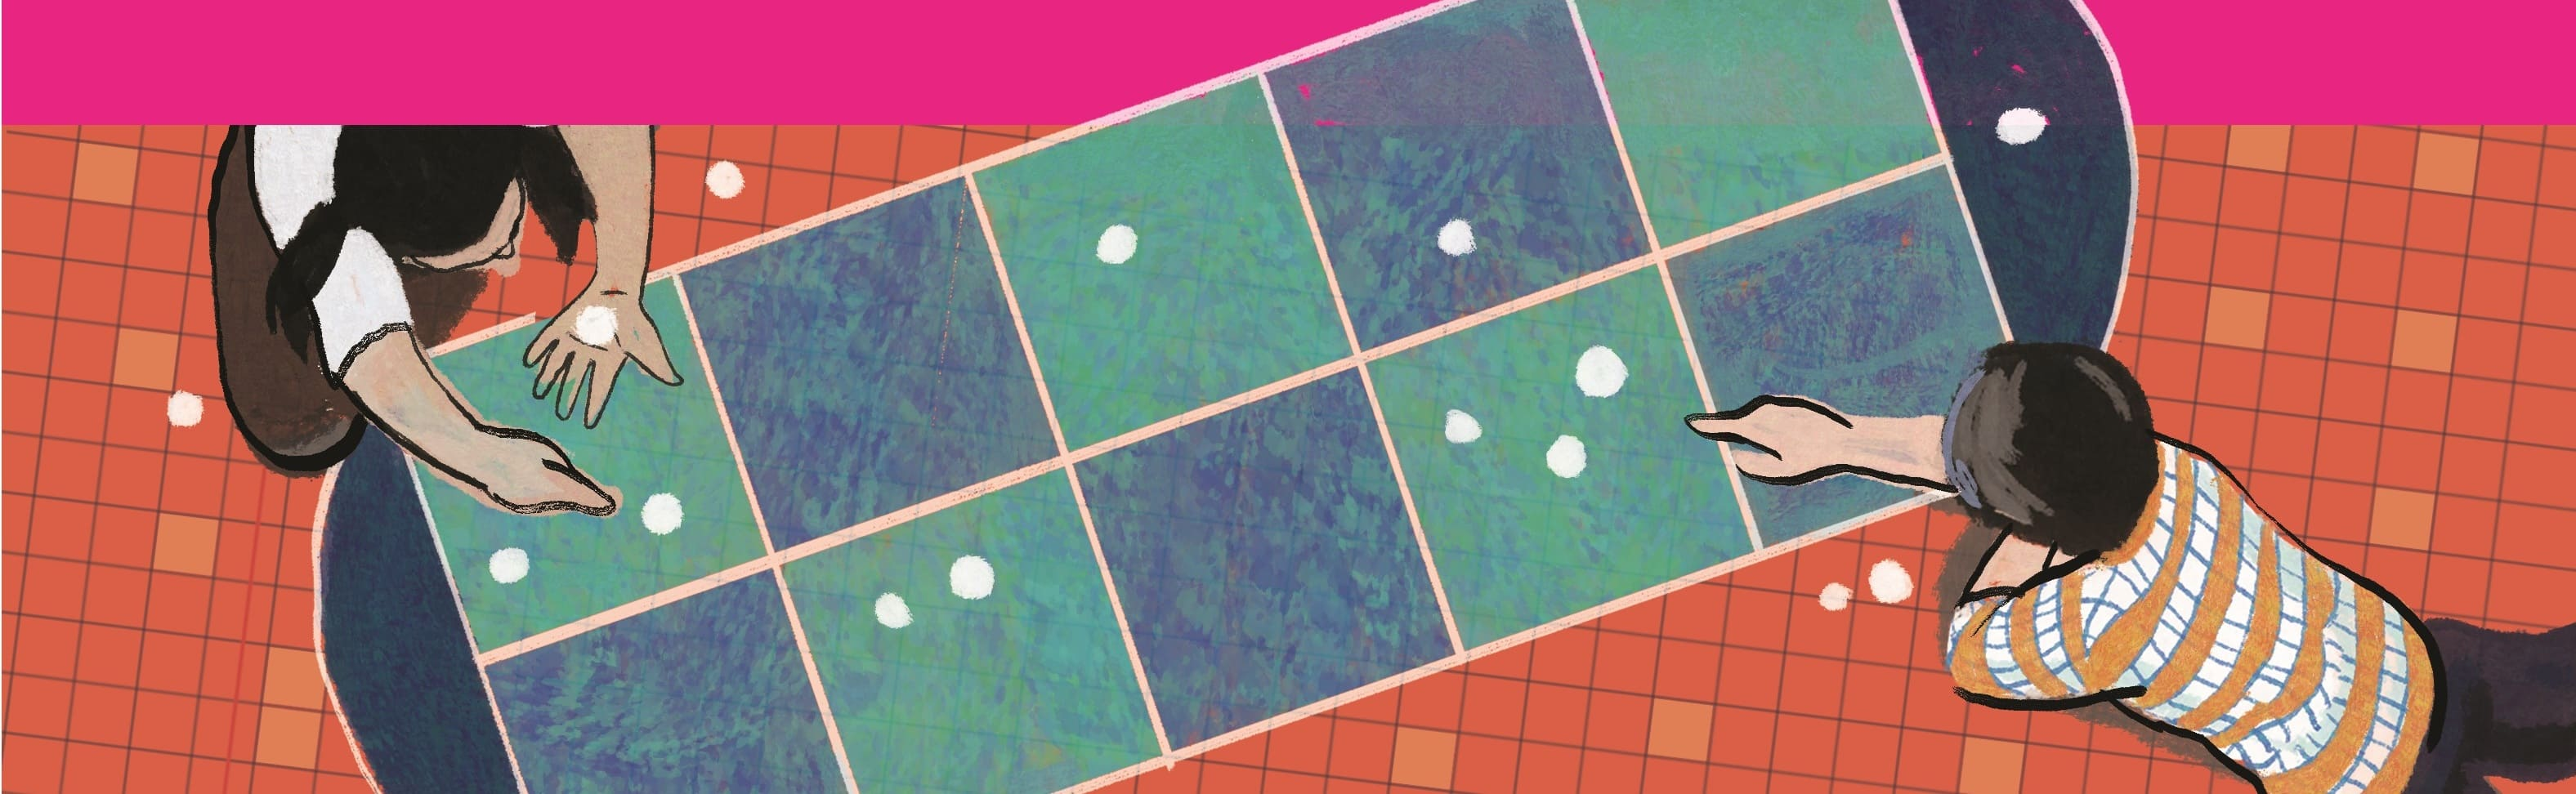
\includegraphics[width=19.3cm]{../bannertoancuabi}}}  
\AddToShipoutPicture*{\put(48,552){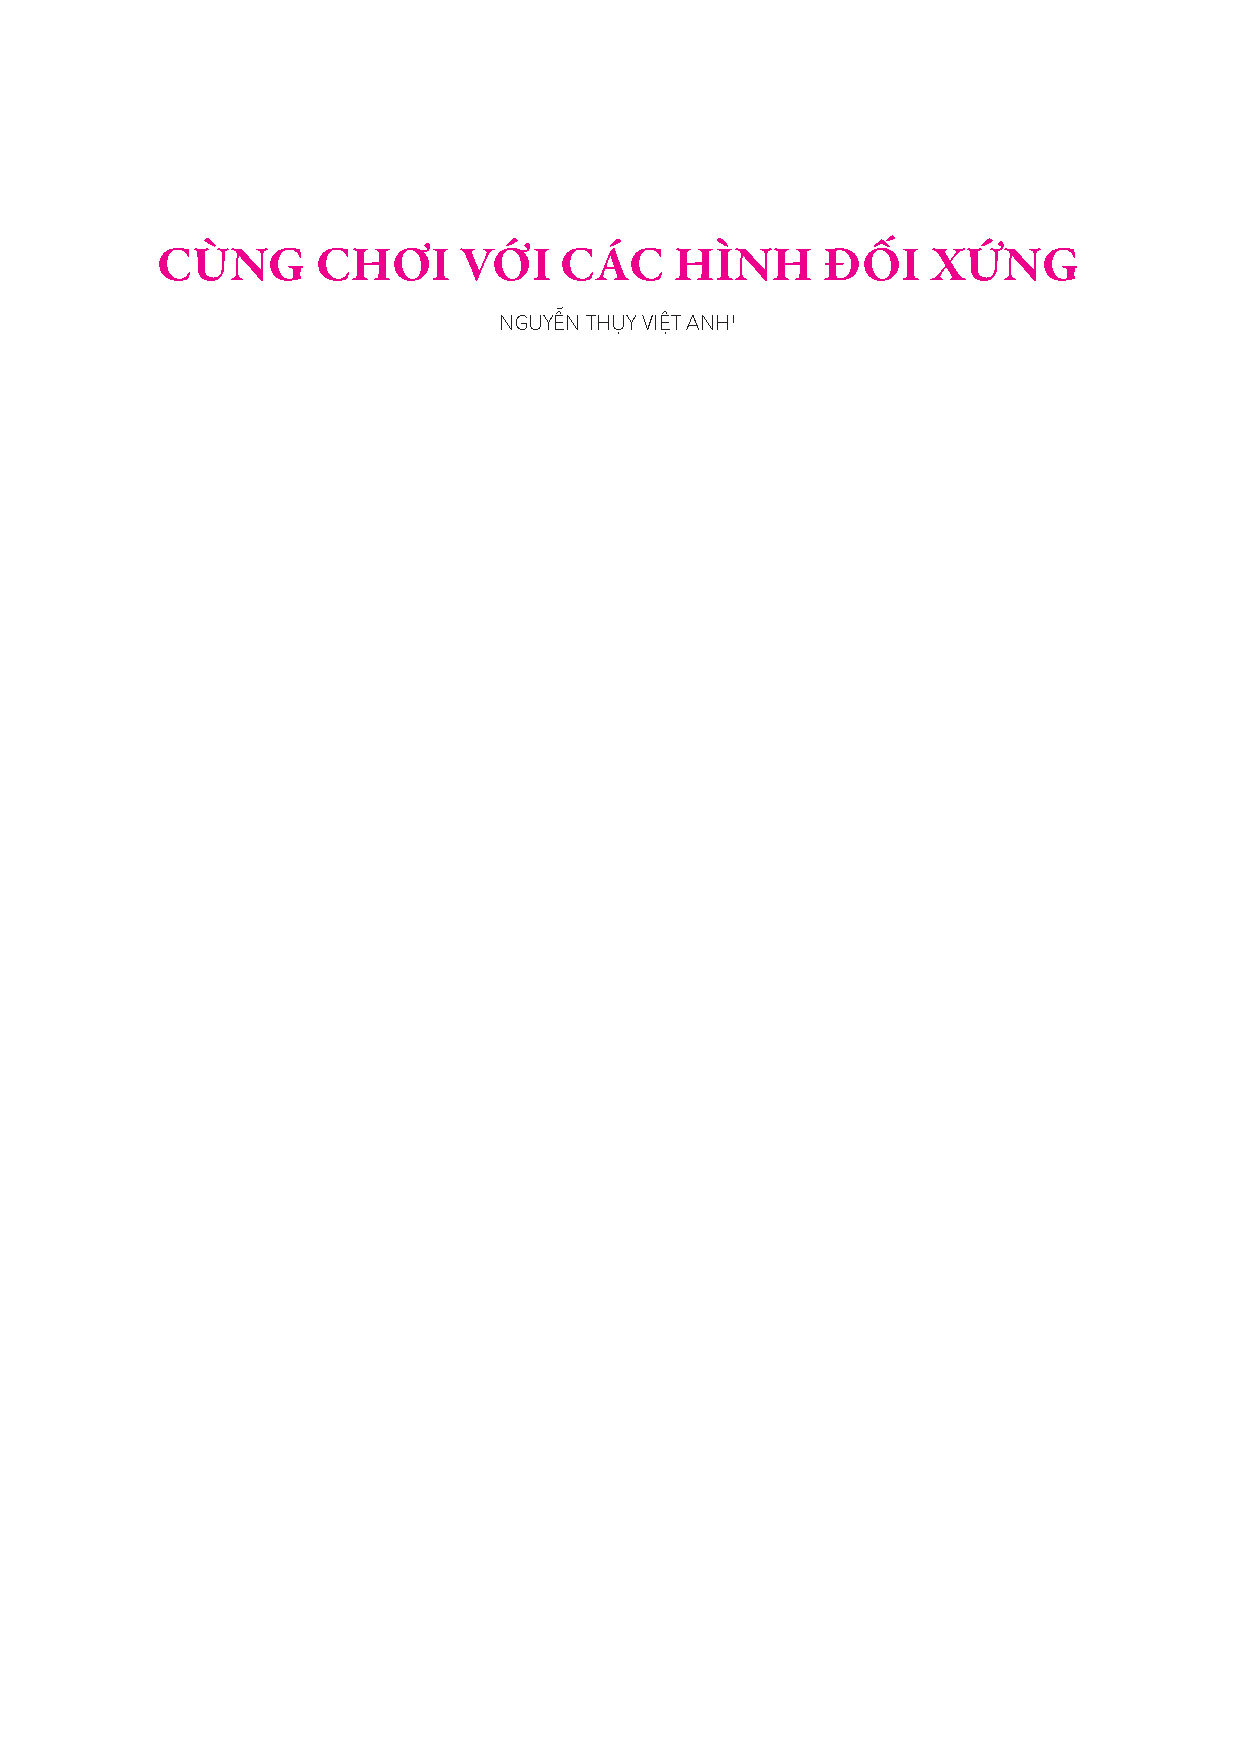
\includegraphics[scale=1]{../tieude10.pdf}}}  
\centering
\endgroup
\vspace*{155pt} 

\begin{multicols}{2}
	Chuồn chuồn tre là sản phẩm độc đáo được các nghệ nhân làng Thạch Xá tạo nên, là món đồ chơi tuổi thơ rất đỗi thân thuộc đối với mỗi người dân trong làng. Lịch sử làng chuồn chuồn tre Thạch Xá với nhiều năm trong nghề đã biến mảnh đất này thành một trong những làng nghề nổi tiếng ở Hà Nội được nhiều du khách biết đến.
	\vskip 0.1cm 
	\begin{center}
		\textit{Chuồn chuồn có cánh thì bay\\
	Có thằng cu Tí thò tay bắt chuồn}
	\end{center}
	\hfill \textit{(Đồng dao, thơ ca dân gian)}
	\begin{figure}[H]
		\vspace*{-5pt}
		\centering
		\captionsetup{labelformat= empty, justification=centering}
		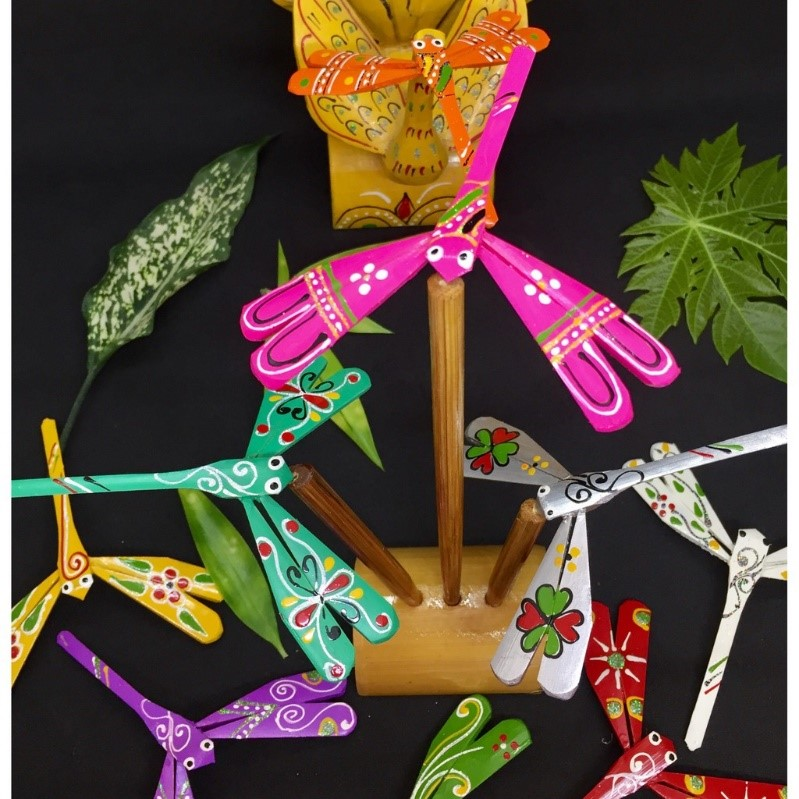
\includegraphics[width= 0.9\linewidth]{10}
		\caption{\small\textit{\color{toancuabi}Ảnh : Internet.}}
		\vspace*{-10pt}
	\end{figure}
	Ngày hôm nay chúng ta sẽ cùng nhau thử sức làm chuồn chuồn tre nhé! Để đơn giản hơn thì chúng ta sẽ thay thế vật liệu để làm chuồn chuồn tre là từ những cây tre thành que kem hoặc giấy.
	\vskip 0.1cm
	\textbf{\color{toancuabi}Cách $\pmb{1}$: Chuồn chuồn que kem thăng bằng}
	\vskip 0.1cm
	\textit{Chuẩn bị nguyên liệu}: 
	\vskip 0.05cm
	-- Các que kem.
	\vskip 0.05cm
	-- Keo, súng bắn keo.
	\vskip 0.05cm
	-- Đũa dùng một lần.
	\vskip 0.05cm
	-- Thước thẳng.
	\vskip 0.05cm
	-- Dao rọc giấy.
	\vskip 0.05cm
	-- Bút chì.
	\vskip 0.05cm
	\textit{Cách làm chuồn chuồn que kem thăng bằng}:
	\vskip 0.1cm
	\textit{Bước} $1$: Sử dụng súng bắn keo dính hai que kem dài $4$ cm lại với nhau.
	\begin{figure}[H]
		\vspace*{-5pt}
		\centering
		\captionsetup{labelformat= empty, justification=centering}
		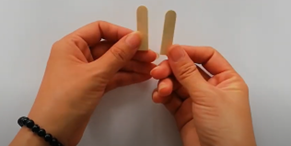
\includegraphics[width=0.7\linewidth]{11}
		
		\vspace*{1pt}
		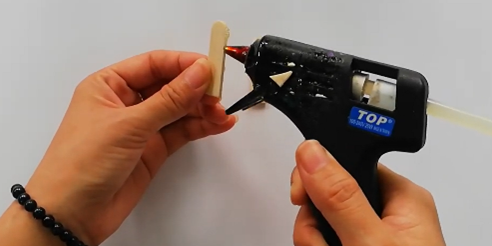
\includegraphics[width=0.7\linewidth]{12}
		
		\vspace*{1pt}
		\hspace*{1pt}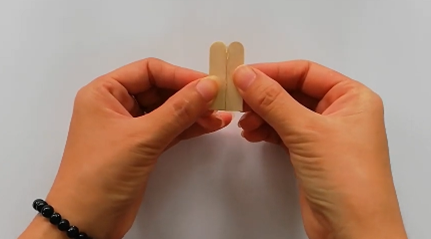
\includegraphics[width=0.7\linewidth]{13}
%		\vspace*{-5pt}
	\end{figure}
	\textit{Bước} $2$: Sử dụng đầu que kem và bút chì để tạo hình phần đầu cho con chuồn chuồn.
	\begin{figure}[H]
		\vspace*{-5pt}
		\centering
		\captionsetup{labelformat= empty, justification=centering}
		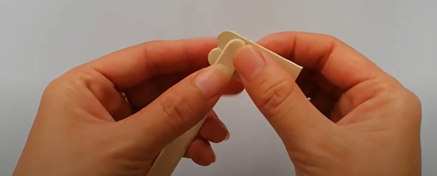
\includegraphics[width=0.7\linewidth]{14}
		
		\vspace*{1pt}
		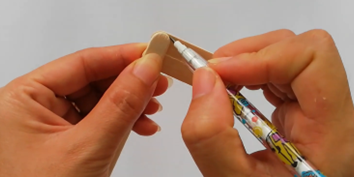
\includegraphics[width=0.7\linewidth]{15}
		
		\vspace*{1pt}
		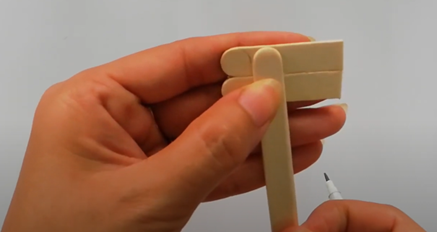
\includegraphics[width=0.7\linewidth]{16}
		
		\vspace*{1pt}
		\hspace*{1pt}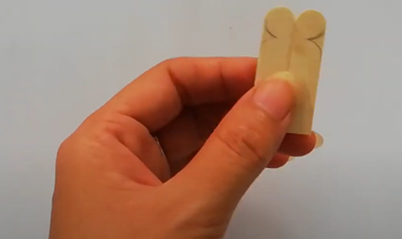
\includegraphics[width=0.7\linewidth]{17}
		\vspace*{-5pt}
	\end{figure}
	\textit{Bước} $3$: Sử dụng dao rọc giấy cắt đi phần khuyết.
	\begin{figure}[H]
		\vspace*{-5pt}
		\centering
		\captionsetup{labelformat= empty, justification=centering}
		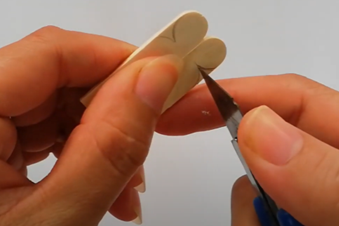
\includegraphics[width=0.7\linewidth]{18}
		
		\vspace*{1pt}
		\hspace*{1pt}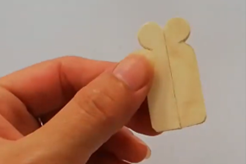
\includegraphics[width=0.7\linewidth]{19}
		\vspace*{-10pt}
	\end{figure}
	\textit{Bước} $4$: Lấy que kem nguyên vẹn rồi cắt chéo đi một nửa (như hình minh họa), sau đó dùng súng bắn keo dán vào que kem dài 10cm để làm cánh chuồn chuồn. (Lưu ý là chuồn chuồn có cánh dài, cánh ngắn).
	\begin{figure}[H]
		\vspace*{5pt}
		\centering
		\captionsetup{labelformat= empty, justification=centering}
		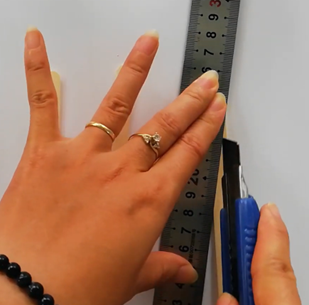
\includegraphics[height=0.35\linewidth]{50}
		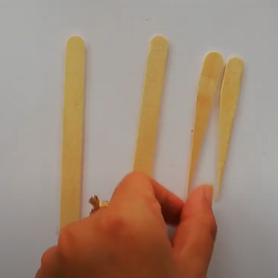
\includegraphics[height=0.35\linewidth]{51}
		
		\vspace*{1pt}
		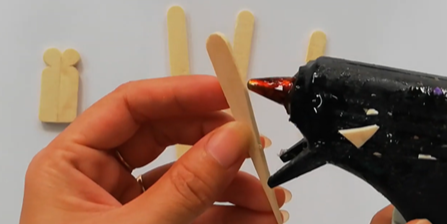
\includegraphics[width=0.7\linewidth]{52}
		
		\vspace*{1pt}
		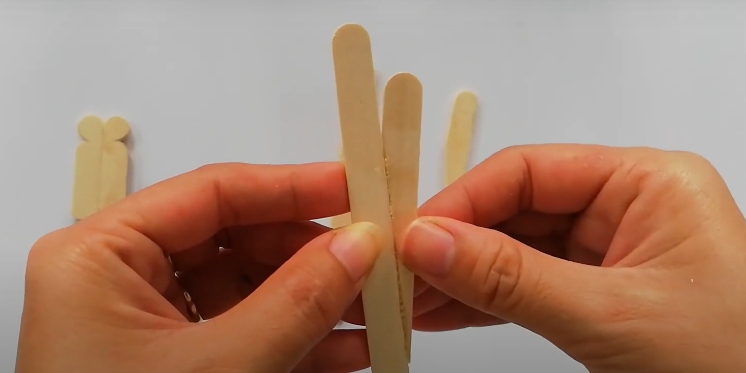
\includegraphics[width=0.7\linewidth]{53}
		
		\vspace*{1pt}
		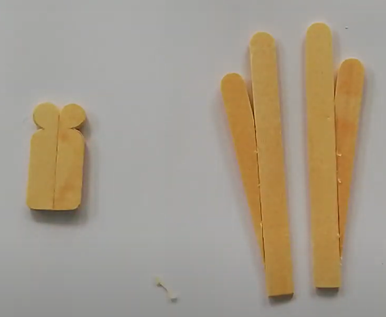
\includegraphics[width=0.7\linewidth]{54}
		\vspace*{-10pt}
	\end{figure}
	\textit{Bước} $5$: Sử dụng súng bắn keo để dán que kem dài $10$ cm vào phần đầu của con chuồn chuồn.
	\begin{figure}[H]
		\vspace*{-5pt}
		\centering
		\captionsetup{labelformat= empty, justification=centering}
		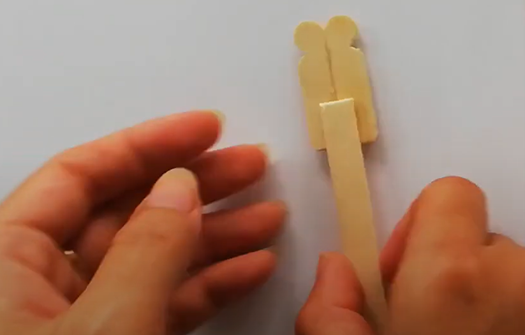
\includegraphics[width=0.7\linewidth]{55}
		\vspace*{-10pt}
	\end{figure}
	\textit{Bước} $6$: Tiếp tục sử dụng súng bắn keo dán hai cánh chuồn chuồn vào thân.
	\begin{figure}[H]
		\vspace*{-5pt}
		\centering
		\captionsetup{labelformat= empty, justification=centering}
		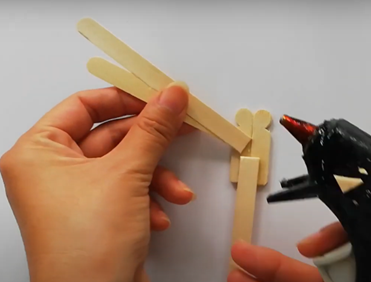
\includegraphics[height=0.36\linewidth]{56}
		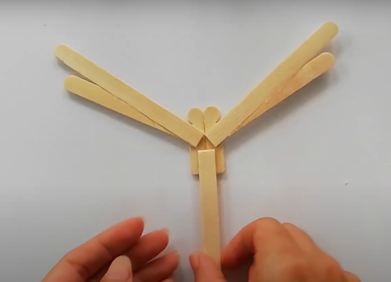
\includegraphics[height=0.36\linewidth]{57}
		\vspace*{-10pt}
	\end{figure}
	\textit{Bước} $7$: Sử dụng súng bắn keo để dán que tre tròn (hoặc đũa dùng một lần) vào chính giữa que kem nguyên vẹn để làm giá đỡ chuồn chuồn.
	\begin{figure}[H]
		\vspace*{5pt}
		\centering
		\captionsetup{labelformat= empty, justification=centering}
		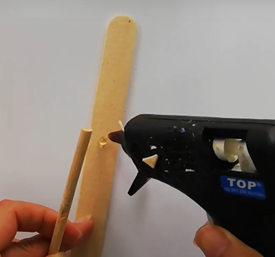
\includegraphics[height=0.34\linewidth]{58}
		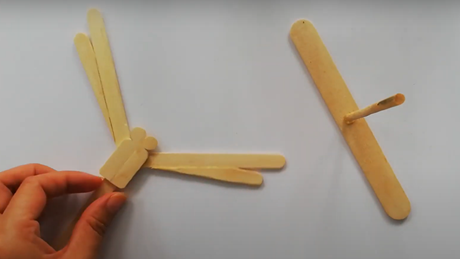
\includegraphics[height=0.34\linewidth]{59}
		\vspace*{-10pt}
	\end{figure}
	Cuối cùng, các em chỉ cần đặt chuồn chuồn lên giá đỡ hoặc lên ngón tay của mình là chuồn chuồn có thể tự thăng bằng được rồi.
	\begin{figure}[H]
		\vspace*{-5pt}
		\centering
		\captionsetup{labelformat= empty, justification=centering}
		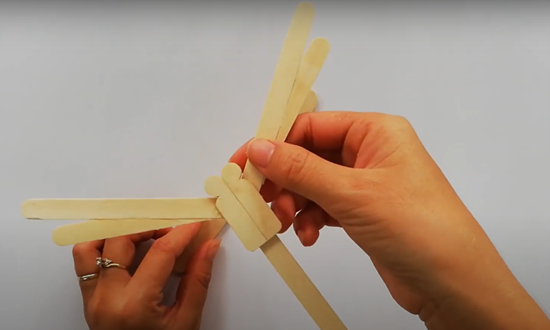
\includegraphics[height=0.35\linewidth]{60}
		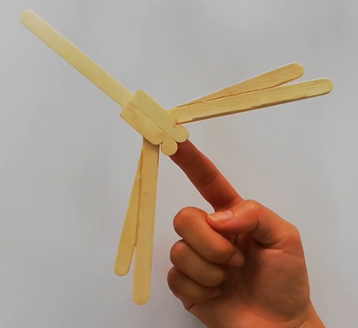
\includegraphics[height=0.35\linewidth]{61}
		\vspace*{-10pt}
	\end{figure}
	\textbf{\color{toancuabi}Cách $\pmb{2}$: Chuồn chuồn giấy thăng bằng}
	\vskip 0.1cm
	\textit{Chuẩn bị nguyên liệu}:
	\vskip 0.1cm
	-- Giấy bìa màu.
	\vskip 0.1cm
	-- Nắp nhựa (tái sử dụng từ chai nhựa bỏ đi).
	\vskip 0.1cm
	-- Đũa dùng một lần.
	\vskip 0.1cm
	-- Bút chì.
	\vskip 0.1cm
	-- Kéo.
	\vskip 0.1cm
	-- Hồ dán.
	\vskip 0.1cm
	-- Keo, súng bắn keo.
	\vskip 0.1cm
	\textit{Cách làm chuồn chuồn giấy thăng bằng}:
	\vskip 0.1cm
	\textit{Bước} $1$: Gấp đôi giấy bìa màu hình chữ nhật (có chiều dài $13$ cm và chiều rộng $4$ cm).
	\begin{figure}[H]
		\vspace*{-5pt}
		\centering
		\captionsetup{labelformat= empty, justification=centering}
		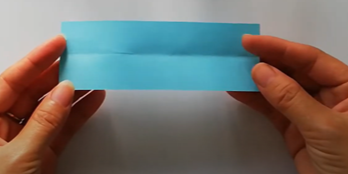
\includegraphics[width=0.7\linewidth]{62}
		
		\vspace*{1pt}
		\hspace*{1pt}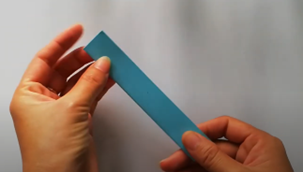
\includegraphics[width=0.7\linewidth]{63}
		\vspace*{-10pt}
	\end{figure}
	\textit{Bước} $2$: Sử dụng bút chì vẽ hình dạng con chuồn chuồn lên tờ giấy màu, sau đó dùng kéo cắt ra.
	\begin{figure}[H]
		\vspace*{5pt}
		\centering
		\captionsetup{labelformat= empty, justification=centering}
		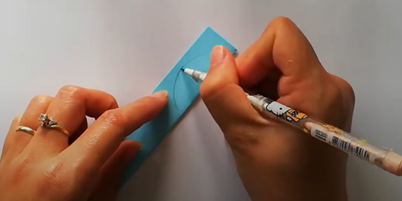
\includegraphics[width=0.7\linewidth]{64}
		
		\vspace*{1pt}
		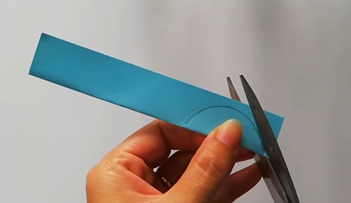
\includegraphics[width=0.7\linewidth]{65}
		
		\vspace*{1pt}
		\hspace*{1pt}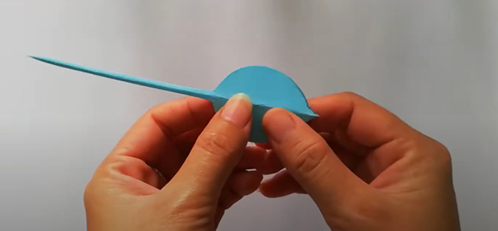
\includegraphics[width=0.7\linewidth]{66}
		\vspace*{-10pt}
	\end{figure}
	\textit{Bước} $3$: Gấp đôi giấy bìa màu hình chữ nhật (có chiều dài $11$ cm và chiều rộng $5$ cm).
	\begin{figure}[H]
		\vspace*{-5pt}
		\centering
		\captionsetup{labelformat= empty, justification=centering}
		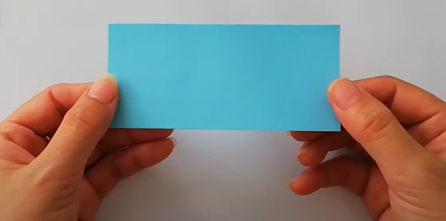
\includegraphics[width=0.7\linewidth]{67}
		
		\vspace*{1pt}
		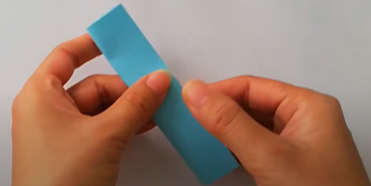
\includegraphics[width=0.7\linewidth]{68}
		\vspace*{-10pt}
	\end{figure}
	\textit{Bước} $4$: Sử dụng bút chì vẽ hình dạng cánh chuồn chuồn lên tờ giấy màu, sau đó dùng kéo cắt ra.
	\begin{figure}[H]
		\vspace*{-5pt}
		\centering
		\captionsetup{labelformat= empty, justification=centering}
		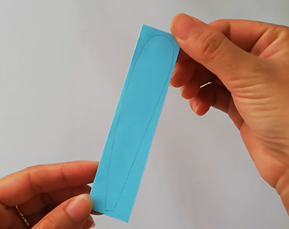
\includegraphics[height=0.31\linewidth]{69}
		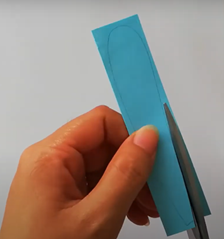
\includegraphics[height=0.31\linewidth]{70}
		
		\vspace*{1pt}
		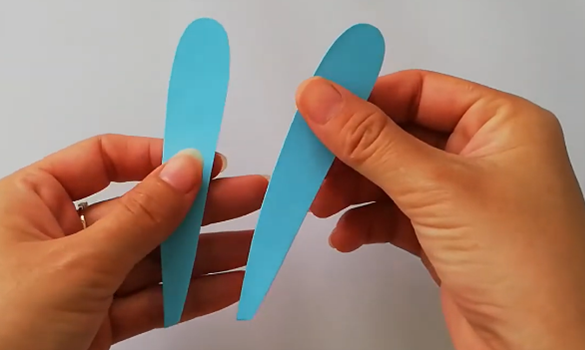
\includegraphics[width=0.7\linewidth]{71}
		\vspace*{-10pt}
	\end{figure}
	\textit{Bước} $5$: Làm tương tự với giấy bìa màu hình chữ nhật (có chiều dài $9$ cm và chiều rộng $4{,}5$~cm) để tạo ra hai cánh nhỏ hơn cho chuồn chuồn.
	\begin{figure}[H]
		\vspace*{-5pt}
		\centering
		\captionsetup{labelformat= empty, justification=centering}
		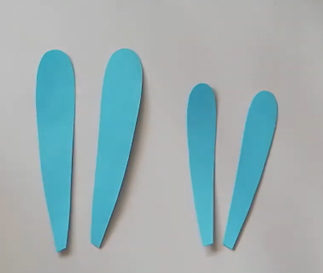
\includegraphics[width=0.7\linewidth]{72}
		\vspace*{-10pt}
	\end{figure}
	\textit{Bước} $6$: Sử dụng hồ dán để dán cánh chuồn chuồn vào thân chuồn chuồn.
	\begin{figure}[H]
		\vspace*{-5pt}
		\centering
		\captionsetup{labelformat= empty, justification=centering}
		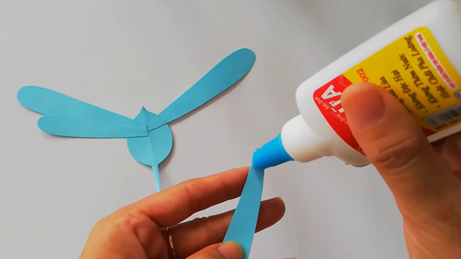
\includegraphics[width=0.7\linewidth]{73}
		\vspace*{-10pt}
	\end{figure}
	\textit{Bước} $7$: Sử dụng súng bắn keo để dán que tre tròn (hoặc đũa dùng một lần) vào chính giữa nắp nhựa để làm giá đỡ chuồn chuồn.
	\begin{figure}[H]
		\vspace*{-5pt}
		\centering
		\captionsetup{labelformat= empty, justification=centering}
		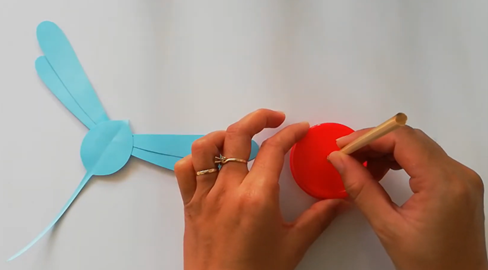
\includegraphics[width=0.7\linewidth]{74}
		\vspace*{-10pt}
	\end{figure}
	Cuối cùng, đặt chuồn chuồn giấy lên giá đỡ hoặc lên ngón tay của mình là chuồn chuồn có thể tự thăng bằng được rồi.
	\begin{figure}[H]
		\vspace*{-5pt}
		\centering
		\captionsetup{labelformat= empty, justification=centering}
		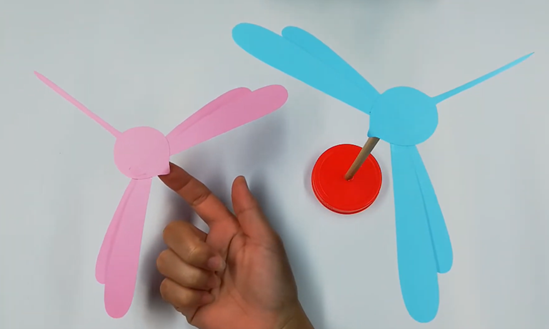
\includegraphics[width=0.7\linewidth]{75}
		\vspace*{-10pt}
	\end{figure}
\end{multicols}

%\begin{multicols}{2}
%	Thám tử Xuân Phong cùng thanh tra Lê Kính tham gia một buổi giới thiệu sản phẩm của hai công ty là Tae Yeon và Tea Yon tại triển lãm Điện tử Expo -- New Vision của khu vực. Công ty  Tae Yeon có uy tín từ lâu đời, với những sản phẩm tinh tế có chất lượng tốt nổi tiếng,  các nhân viên của công ty luôn nói thật. Còn công ty Tea Yon chuyên sản xuất đồ rẻ, kém chất lượng, bắt chước kiểu dáng của công ty Tae Yeon nên Ban giám đốc dặn các nhân viên của mình chỉ được nói dối trong buổi triển lãm. 
%	\vskip 0.1cm
%	Vừa đặt chân tới khu vực triển lãm được trang hoàng lộng lẫy, Xuân Phong gặp ngay $5$ đại diện  của hai công ty này đứng tại cổng ra vào và tươi cười niềm nở tiếp đón. Xuân Phong tiến tới họ và hỏi cả $5$ người cùng một câu hỏi ``Có bao nhiêu người đến từ công ty Tae Yeon trong số các bạn?" 
%	\vskip 0.1cm
%	Người thứ nhất trả lời ``Không có ai cả". Hai người tiếp theo đều trả lời ``Có đúng một người". 
%	\vskip 0.1cm
%	Vậy hai người còn lại sẽ trả lời câu hỏi của thám tử Xuân Phong như thế nào nhỉ? Em có thể suy đoán ra câu trả lời của họ và giải thích lập luận được không?
%	\begin{figure}[H]
	%		\centering
	%		\vspace*{-5pt}
	%		\captionsetup{labelformat= empty, justification=centering}
	%		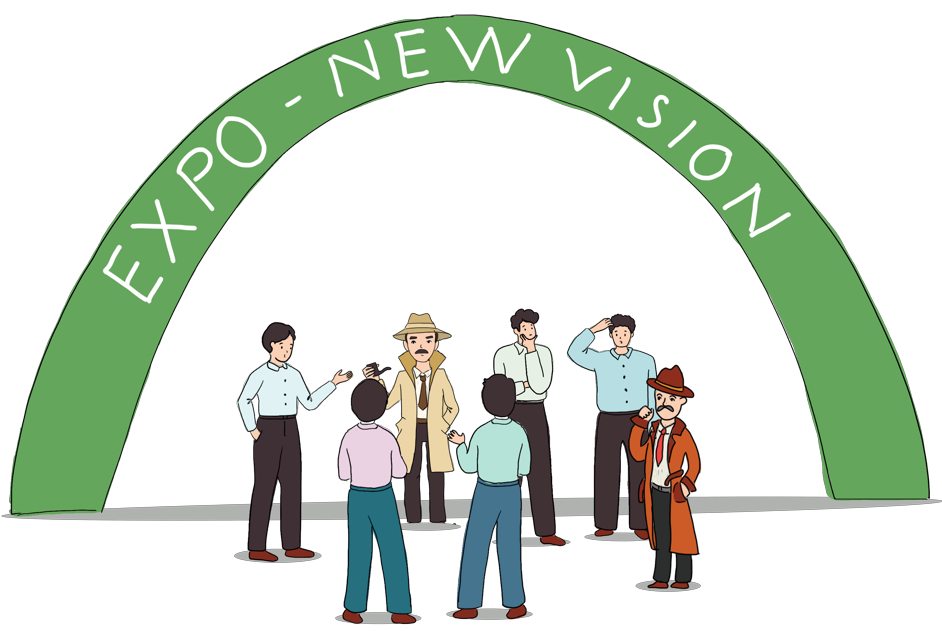
\includegraphics[width=1\linewidth]{xuanphong}
	%		\vspace*{-5pt}
	%	\end{figure}
%\end{multicols}
%\vspace*{-10pt}
%{\color{toancuabi}\rule{1\linewidth}{0.1pt}}
%\begingroup
%\AddToShipoutPicture*{\put(115,190){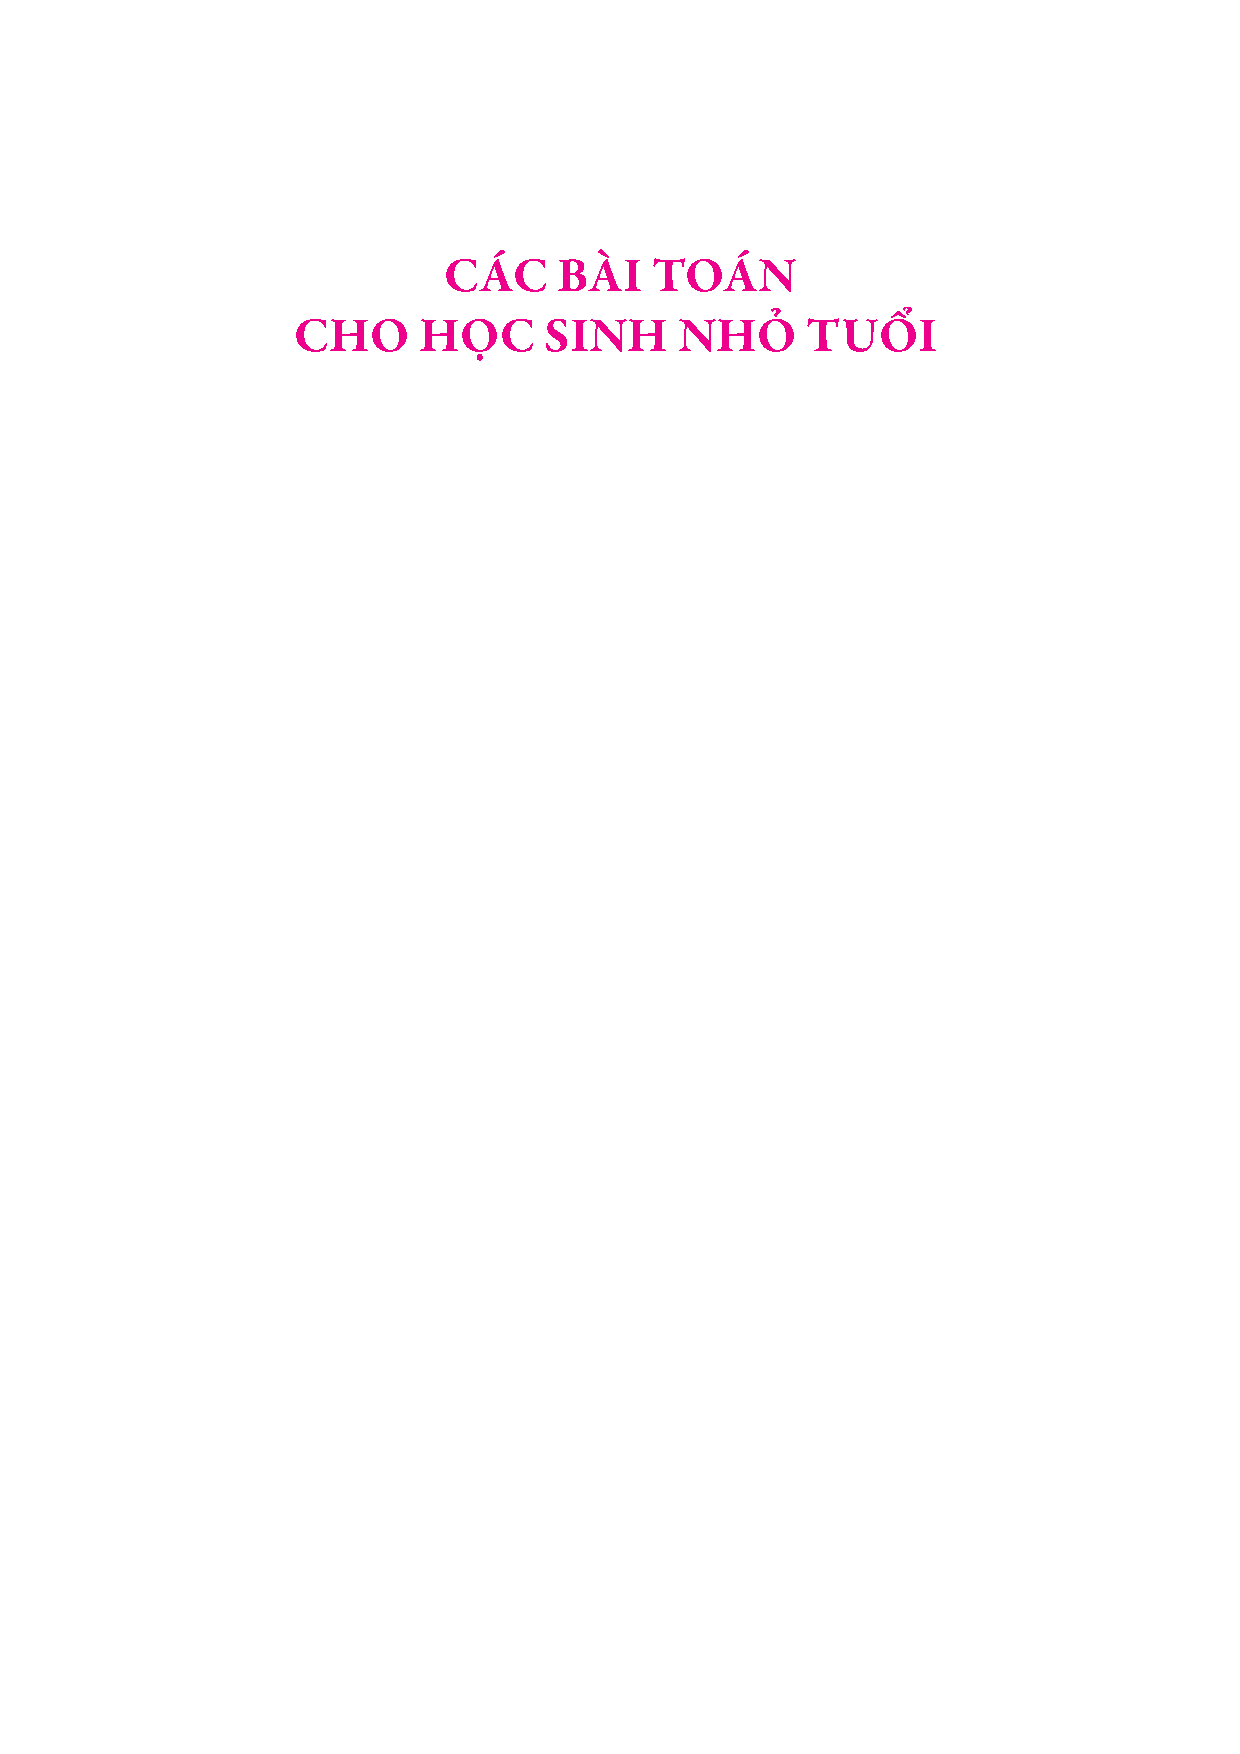
\includegraphics[scale=1]{../tieude11.pdf}}} 
%\centering
%\endgroup
%\vspace*{50pt}
%
%\begin{multicols}{2}
%	$\pmb{1.}$	Trong một cuộc thi thể thao, ban tổ chức chọn ra một số bạn học sinh ở lớp $5A$ và một số bạn ở lớp $5B$ thi đấu trực tiếp. Mỗi bạn ở lớp $5A$ được chọn ra sẽ thi đấu duy nhất một trận với một bạn ở lớp $5B$, và ngược lại, mỗi bạn ở lớp $5B$ được chọn ra chỉ đấu đúng một trận với một bạn ở lớp $5A$.
%	\begin{figure}[H]
	%		\centering
	%		\vspace*{-5pt}
	%		\captionsetup{labelformat= empty, justification=centering}
	%		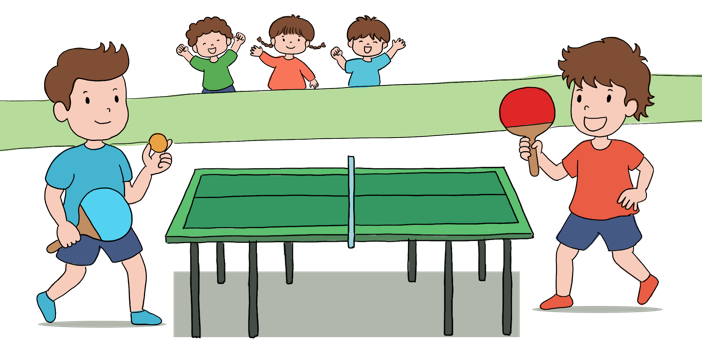
\includegraphics[width=1\linewidth]{Pi5_bai1}
	%		\vspace*{-15pt}
	%	\end{figure}
%	Biết rằng số học sinh lớp $5A$ được chọn thi đấu chiếm $2/3$ tổng số học sinh toàn lớp $5A$, còn số học sinh lớp $5B$ được chọn thi đấu chiếm $3/5$ tổng số học sinh toàn lớp $5B$. Tổng số học sinh của cả hai lớp là $57$ bạn. Hỏi có bao nhiêu học sinh của hai lớp đã tham gia các trận thi đấu trực tiếp?
%	
%	$\pmb{2.}$ Công ty vận tải được thông báo ngắn gọn là có một số kiện hàng có tổng khối lượng là $10$ tấn cần được vận chuyển, hơn nữa mỗi kiện hàng nặng không quá $1$ tấn. Hỏi công ty  cần điều động ít nhất bao nhiêu xe tải có trọng tải là $3$ tấn mỗi xe để luôn chắc chắn chở được hết được số hàng hoá đó?
%	\begin{figure}[H]
	%		\centering
	%		\vspace*{-10pt}
	%		\captionsetup{labelformat= empty, justification=centering}
	%		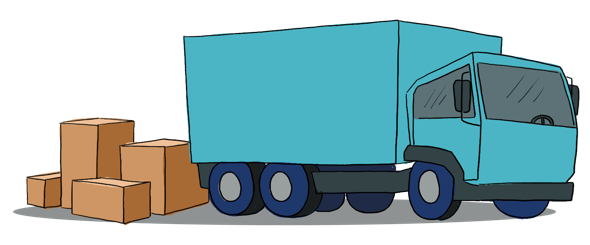
\includegraphics[width=0.8\linewidth]{Pi5_bai2}
	%		\vspace*{-15pt}
	%	\end{figure}
%	$\pmb{3.}$ Sau khi được sạc đầy pin, điện thoại di động của bạn An dùng đúng $6$ tiếng ở chế độ trò chuyện hoặc đúng $210$ tiếng ở chế độ chờ. Khi bạn An lên tàu hoả để đi du lịch, pin của bạn được sạc đầy $100\%$, và trên tàu không có ổ cắm sạc nên khi xuống ga, pin của bạn cũng vừa hết sạch. Biết rằng An đã nói chuyện với bạn bè đúng một nửa thời gian khi ngồi trên tàu, còn nửa thời gian còn lại đặt điện thoại ở chế độ chờ. Hỏi thời gian An đi trên tàu hoả là bao nhiêu lâu?
%	\begin{figure}[H]
	%		\centering
	%		\vspace*{-5pt}
	%		\captionsetup{labelformat= empty, justification=centering}
	%		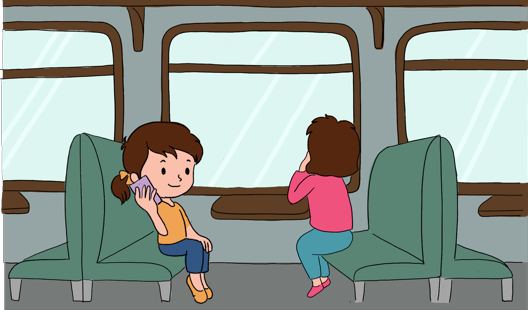
\includegraphics[width=0.85\linewidth]{Pi5_bai3}
	%		\vspace*{-10pt}
	%	\end{figure}
%	$\pmb{4.}$ Một nhóm học sinh đi bộ từ điểm hẹn tới bến xe buýt để kịp đón chuyến xe vào lúc $8$ giờ. Cũng vào thời điểm này, từ điểm tham quan, một chiếc xe buýt cũng xuất phát để tới kịp bến xe đón nhóm học sinh đó. Tuy  nhiên nhóm học sinh tới bến xe buýt khá sớm, vào lúc $6$ giờ $10$ phút, nên họ quyết định đi bộ tiếp tới điểm tham quan. Trên đường, các bạn đã gặp được xe buýt và lên xe đi tiếp.  Cuối cùng cả nhóm đến được điểm tham quan sớm hơn $20$ phút so với thời gian ấn định. Biết rằng vận tốc của xe buýt là $60$ km/h và vận tốc đi bộ của các em học sinh luôn không đổi. Hãy tìm vận tốc đi bộ của nhóm học sinh trước khi gặp xe buýt.
%	\begin{figure}[H]
	%		\centering
	%		\vspace*{-10pt}
	%		\captionsetup{labelformat= empty, justification=centering}
	%		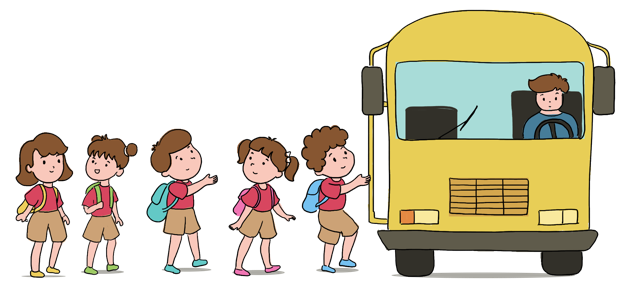
\includegraphics[width=0.85\linewidth]{Pi5_bai4}
	%		\vspace*{-10pt}
	%	\end{figure}
%	$\pmb{5.}$ 	Có $100$ chiếc xe ô tô đỗ liền nhau thành một hàng dọc bên lề đường, trong đó có $70$ chiếc xe hiệu Mercedes, còn lại là những xe nhãn hiệu khác. Trong các xe nhãn hiệu Mercedes có $30$ chiếc màu đỏ, $20$ chiếc màu vàng và $20$ chiếc màu hồng. Biết rằng không có hai xe Mercedes nào khác màu lại đỗ cạnh nhau. Em hãy chỉ ra rằng luôn tìm ra $3$ chiếc xe Mercedes cùng màu đỗ liên tiếp nhau.
%	\begin{figure}[H]
	%		\centering
	%		\vspace*{-5pt}
	%		\captionsetup{labelformat= empty, justification=centering}
	%		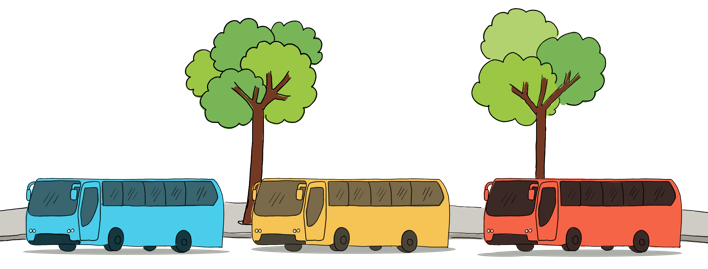
\includegraphics[width=0.85\linewidth]{Pi5_bai5}
	%		\vspace*{-10pt}
	%	\end{figure}
%	$\pmb{6.}$ Một lớp học có $20$ em học sinh. Cô giáo chủ nhiệm của lớp tổ chức một số buổi tham quan vào mỗi ngày cuối tuần trong suốt năm học, mỗi buổi tham quan có ít nhất $4$ em học sinh tham gia. Em hãy chứng minh rằng có một buổi tham quan mà mỗi em học sinh tham gia buổi đó đều tham gia ít nhất $1/17$ tổng số tất cả các buổi tham quan của cả năm học.
%	\begin{figure}[H]
	%		\centering
	%		\vspace*{-15pt}
	%		\captionsetup{labelformat= empty, justification=centering}
	%		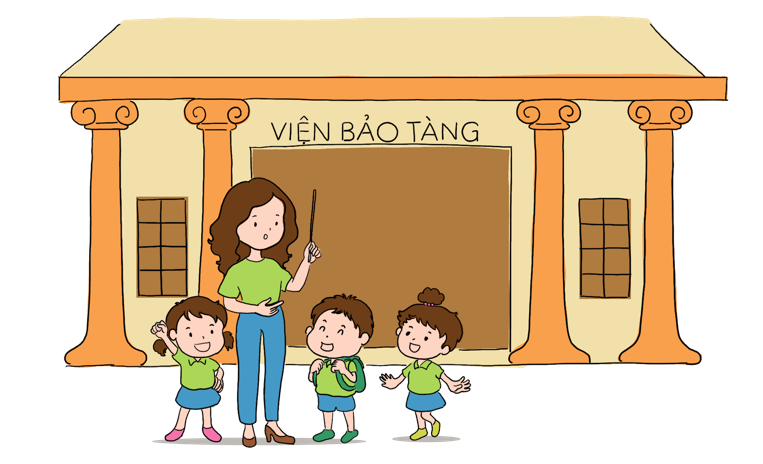
\includegraphics[width=0.8\linewidth]{Pi5_bai6}
	%		%		\vspace*{-5pt}
	%	\end{figure}
%\end{multicols}
%\newpage
%\begingroup
%\AddToShipoutPicture*{\put(110,645){
\includegraphics[scale=1]{../tieude2.pdf}}} 
%\centering
%\endgroup
%\vspace*{55pt}
%
%\begin{multicols}{2}
%	$\pmb{1.}$ Một bác nông dân chở một xe ô tô quất cảnh ra chợ Tết để bán. Sau khi bán hết cây quất cuối cùng với giá $230$ nghìn đồng, bác tính nhẩm lại thấy mình đã bán số cây quất với giá trung bình là $245$ nghìn đồng/cây. Nhưng ngay lúc ấy người mua cây quất cuối quay trở lại và chỉ cho bác thấy cành quất bị rụng quá nhiều lá, nên ông ta chỉ đồng ý mua với giá $158$ nghìn đồng. 
%	Bác chấp thuận và bán cây quất đó. Khi nhẩm tính lại, bác nông dân thấy giá trung bình của xe quất bây giờ là $242$ nghìn đồng/cây. Hỏi bác đã bán được bao nhiêu cây quất?
%	\begin{figure}[H]
	%		\centering
	%		\vspace*{-10pt}
	%		\captionsetup{labelformat= empty, justification=centering}
	%		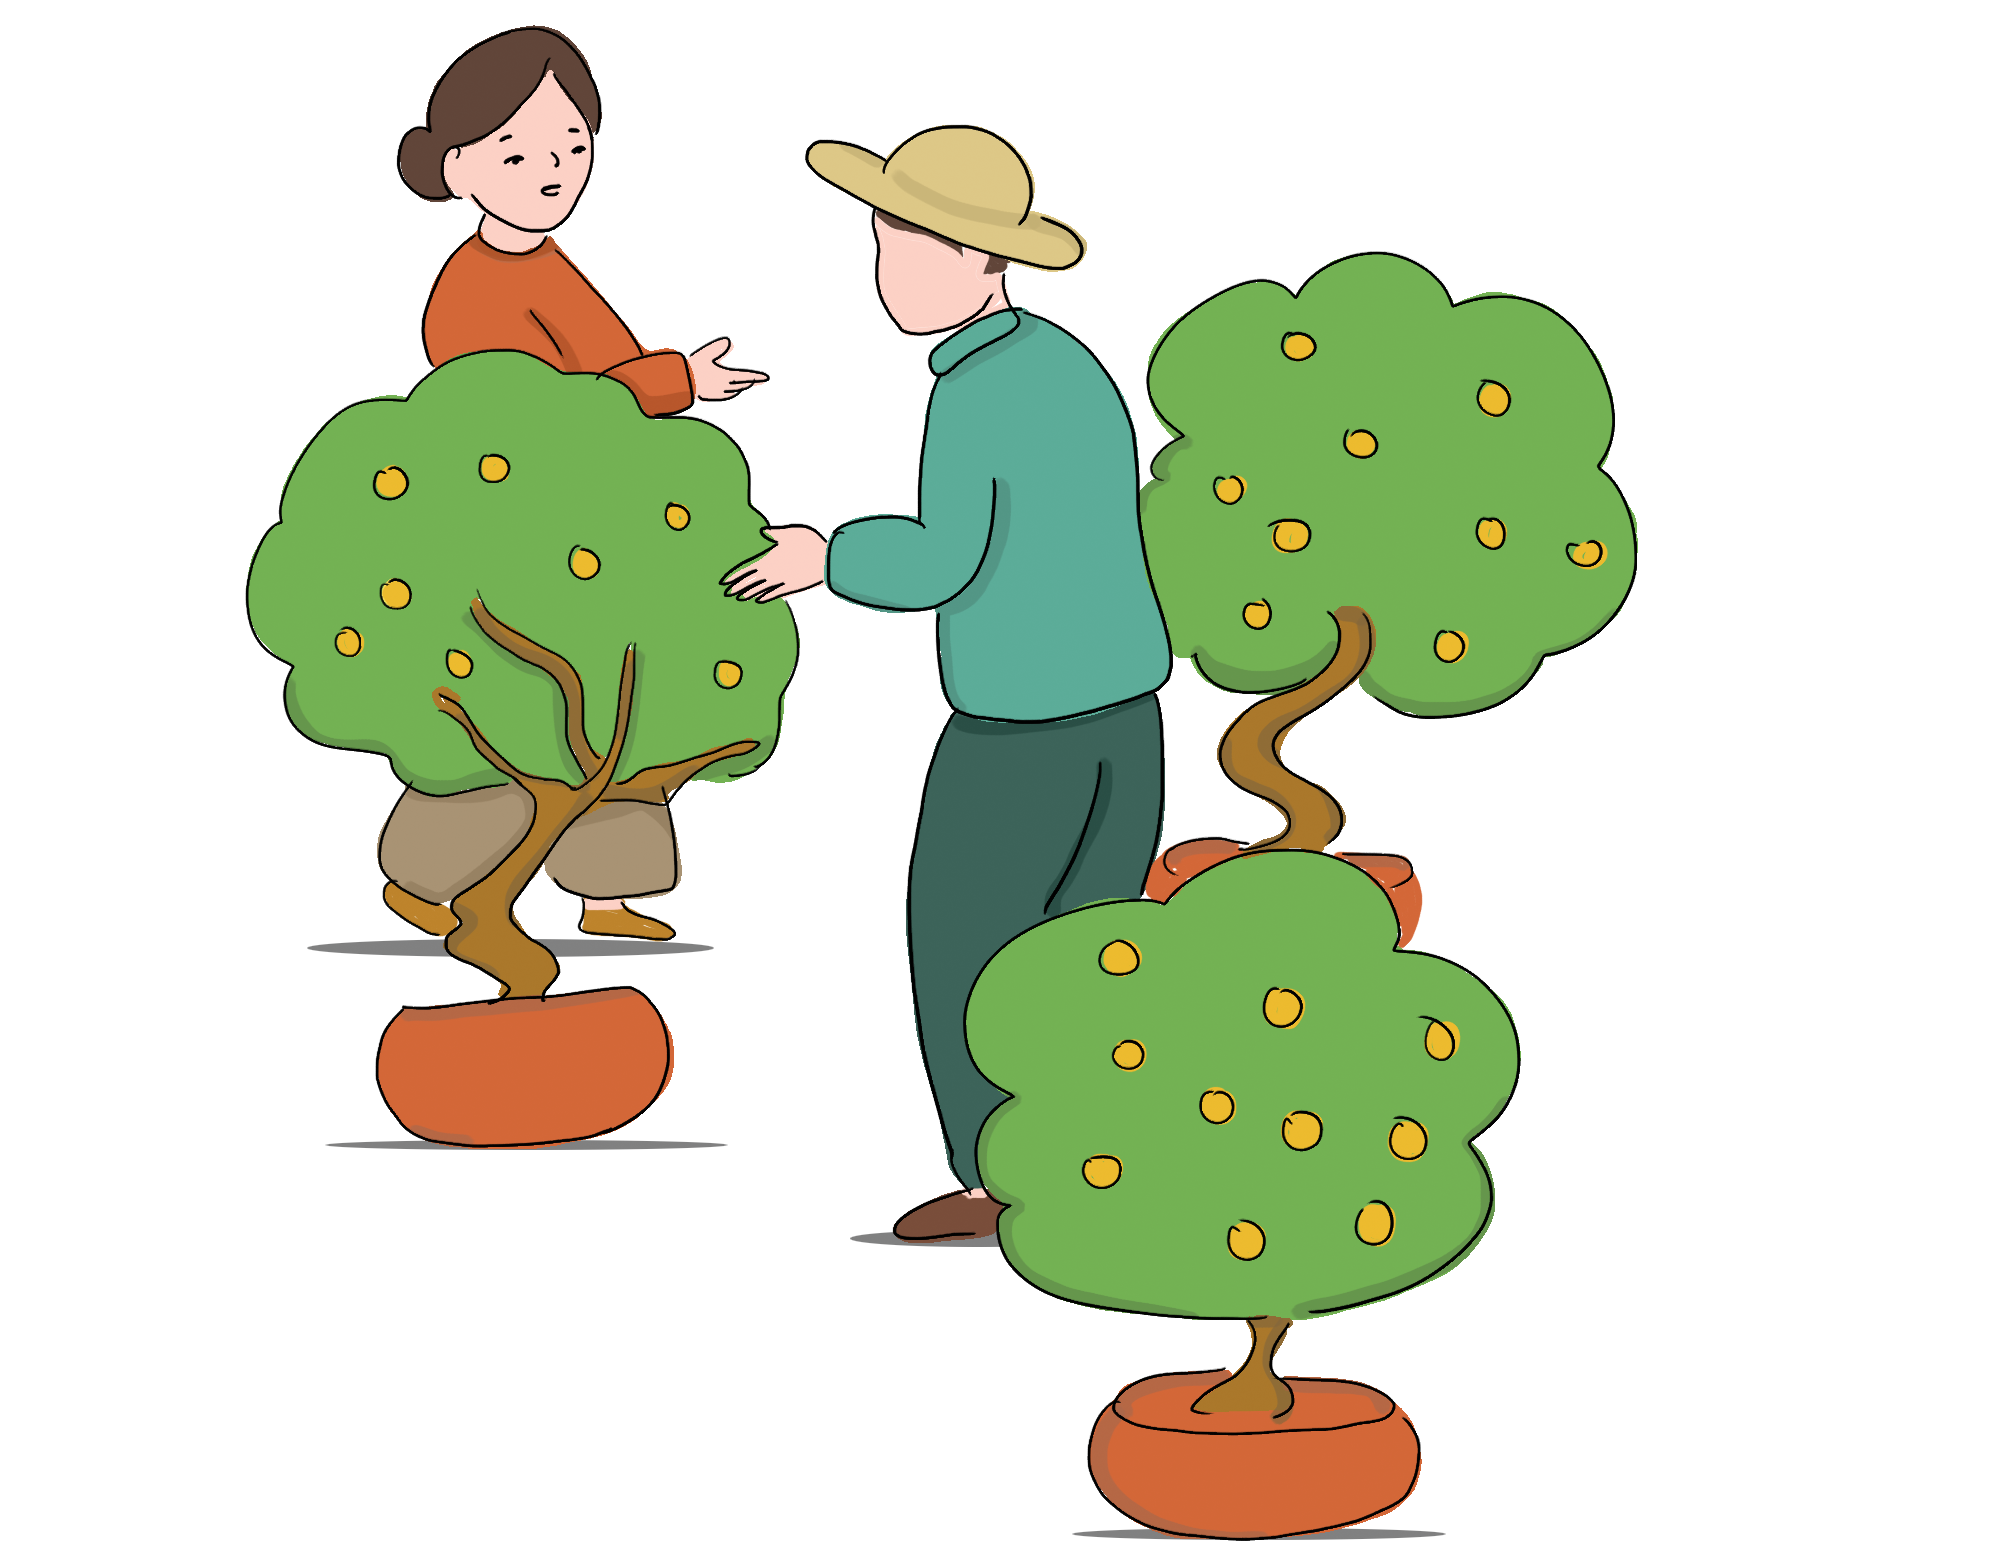
\includegraphics[width=0.7\linewidth]{Pi1_2_Bai1}
	%		\vspace*{-15pt}
	%	\end{figure}
%	\textit{Lời giải.} Gọi số cây quất là $n$, và tổng số tiền bán được của toàn bộ số quất, trừ cây cuối cùng, là $q$ (nghìn đồng). Khi đó $q+230 = 245n$ và $q+ 158 = 242n$. Trừ hai đẳng thức này ta có $72 = 3n$. Suy ra bác nông dân đã bán được $24$ cây quất.
%	\vskip 0.1cm
%	$\pmb{2.}$ Chuyện kể rằng có một người khi gặp nhà triết học và toán học Hy Lạp Pythagoras đã hỏi ông: ``Bây giờ là mấy giờ?" Pythagoras đã trả lời ``Cho đến hết ngày, còn lại hai lần của hai phần năm khoảng thời gian đã trôi qua từ lúc bắt đầu ngày". Nghe vậy, người đó chịu không thể nghĩ ra ngay được lúc họ gặp nhau là mấy giờ. Em có thể giúp trả lời lúc đó là mấy giờ được không?
%	\vskip 0.1cm
%	\textit{Lời giải.} 	Gọi $x$ là thời gian (tính theo giờ) đã trôi qua từ lúc bắt đầu ngày. Khi đó ta có hệ thức sau theo câu trả lời của Pythagoras: $24 - x = 4/5 x$. Suy ra $x = 40/3$ (giờ), có nghĩa là $13$ giờ $20$ phút. Vậy người đó đã gặp Pythagoras lúc $13$ giờ $20$ phút.
%	\begin{figure}[H]
	%		\centering
	%		\vspace*{-10pt}
	%		\captionsetup{labelformat= empty, justification=centering}
	%		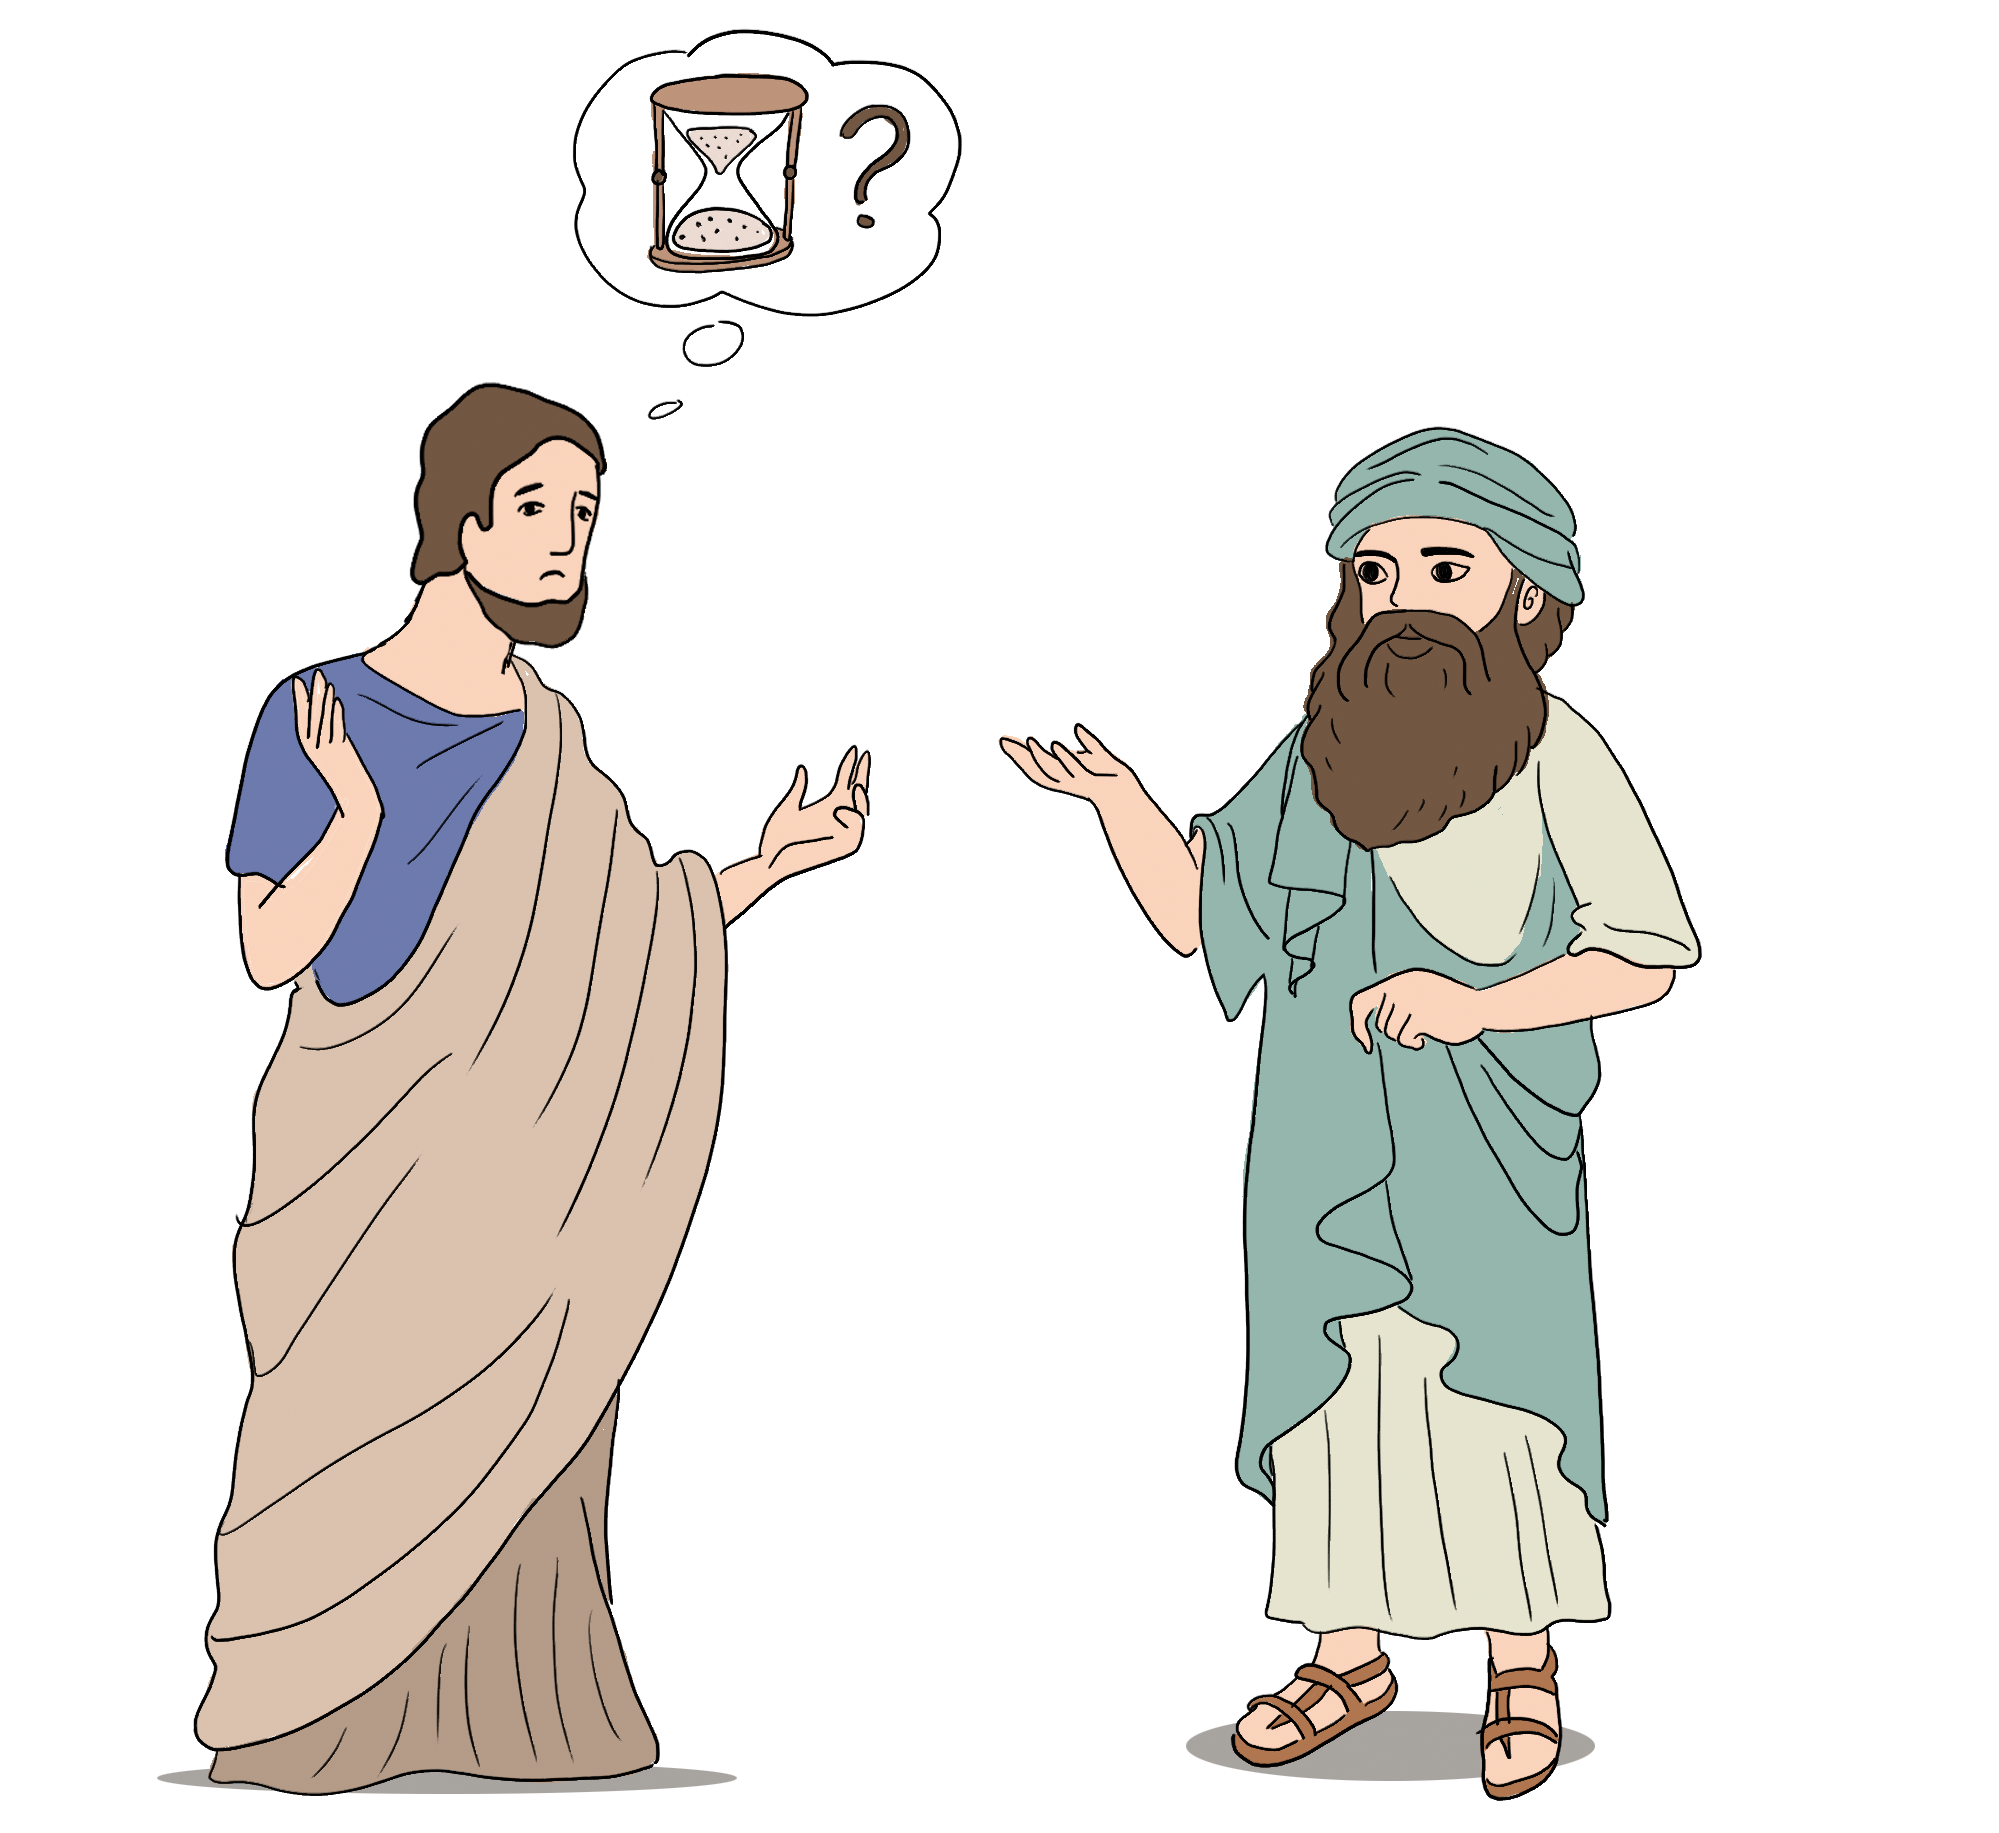
\includegraphics[width=0.6\linewidth]{Pi1_2_Bai2}
	%		\vspace*{-10pt}
	%	\end{figure}
%	$\pmb{3.}$ Một tháng trước bà Hoa ra chợ mua một cân khoai tây, một cân thịt và một chục trứng. Chủ nhật vừa rồi, khoai tây tăng lên gấp $3$, thịt gấp $4$ lần còn trứng đắt gấp $5$ lần, nên bà Hoa phải trả $600$ nghìn cho từng ấy món hàng như lần thứ nhất. Hôm nay thì khoai lại đắt gấp $6$ lần so với tháng trước, thịt đắt gấp $5$ lần còn trứng chỉ đắt gấp $4$ lần nên bà Hoa lại phải trả $660$ nghìn với cùng một lượng hàng. Hỏi bà Hoa đã trả bao nhiêu tiền cho lần mua thứ nhất?
%	\begin{figure}[H]
	%		\centering
	%		\vspace*{-10pt}
	%		\captionsetup{labelformat= empty, justification=centering}
	%		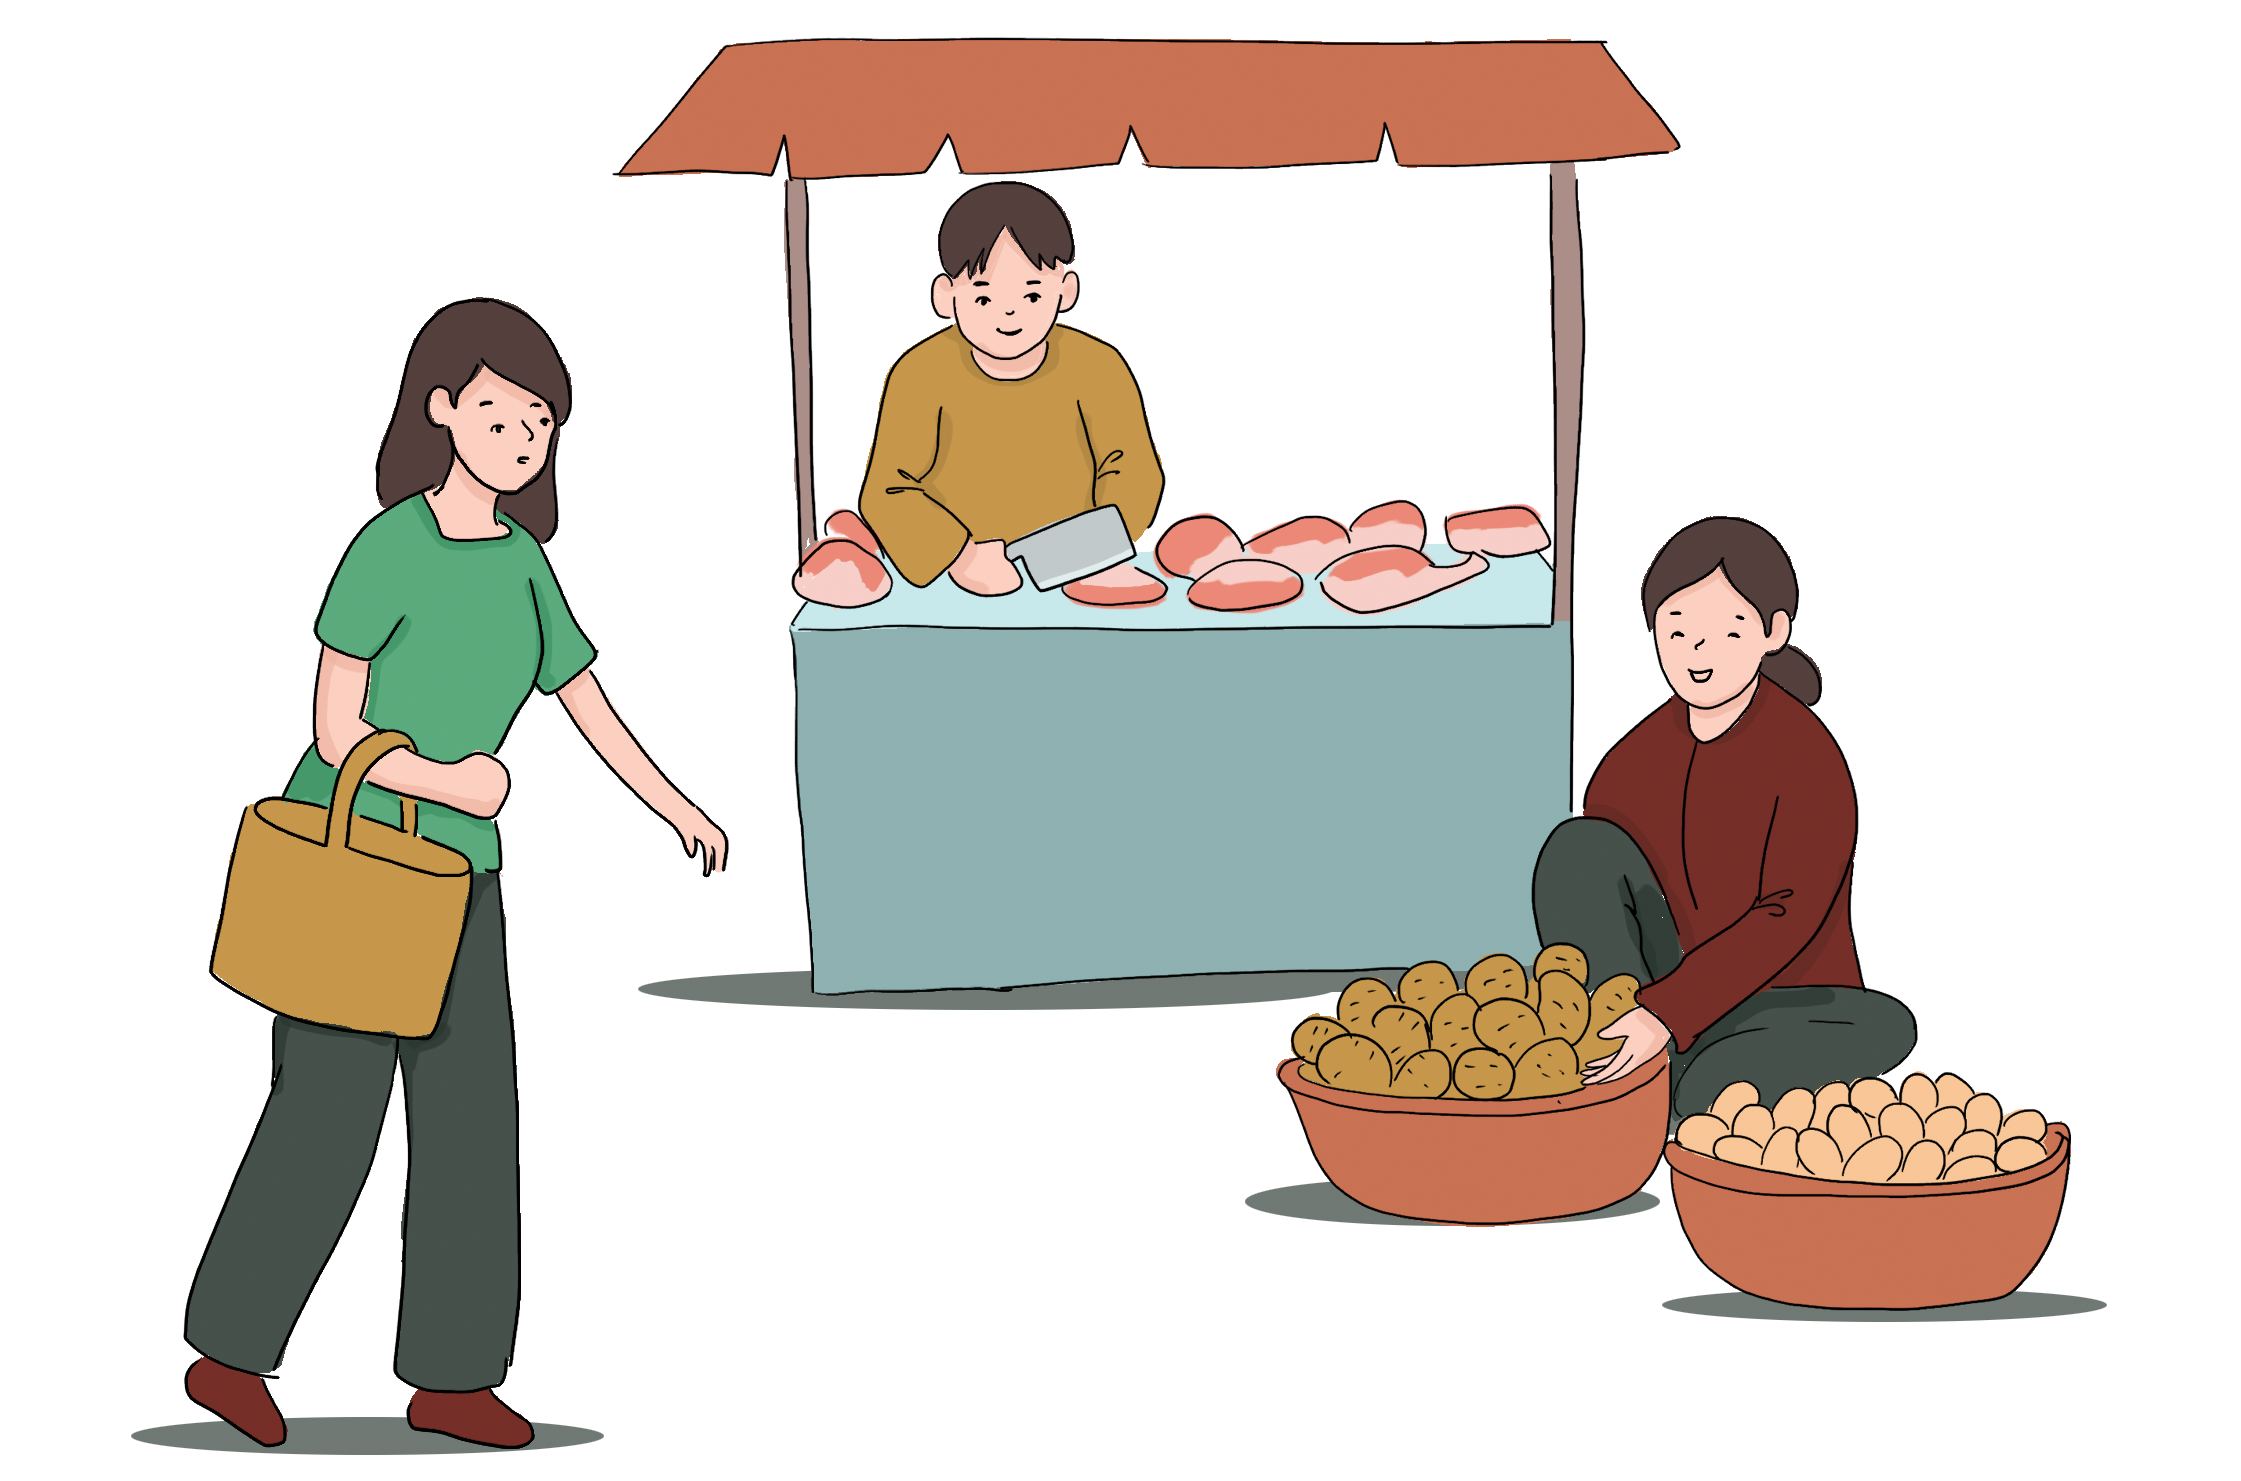
\includegraphics[width=0.6\linewidth]{Pi1_2_Bai3}
	%		\vspace*{-10pt}
	%	\end{figure}
%	\textit{Lời giải.} 	Giả sử vào tháng trước trong lần mua đầu tiên giá một cân khoai tây là $a$ (nghìn đồng), giá một cân thịt là $b$ (nghìn đồng) và giá một chục trứng là $c$ (nghìn đồng). Khi đó trong lần mua thứ nhất bà Hoa đã trả $a + b + c$ (nghìn), trong lần mua thứ hai là $3a+4b+5c = 600$ và trong lần mua thứ ba là $6a + 5b+ 4c = 660$. Cộng hai đẳng thức cuối này, ta có $9(a+b+c)= 1260$. Suy ra $a+b+c = 140$. Vậy vào tháng trước bà Hoa chỉ phải trả có $140$ nghìn đồng.
%	\vskip 0.1cm
%	$\pmb{4.}$ Trong một buổi dạ hội nọ mỗi quý ông đã hân hạnh khiêu vũ với ba quý bà, còn mỗi quý bà cũng đã khiêu vũ với ba quý ông. Em hãy chỉ ra rằng số quý ông và số quý bà tham gia dạ hội là bằng nhau.
%	\begin{figure}[H]
	%		\centering
	%		\vspace*{-5pt}
	%		\captionsetup{labelformat= empty, justification=centering}
	%		\includegraphics[width=0.75\linewidth]{Pi1_2_Bai4}
	%		\vspace*{-10pt}
	%	\end{figure}
%	\textit{Lời giải.} Ta sẽ tính tổng tất cả các cặp đã khiêu vũ với nhau. Một mặt, tổng này sẽ bằng $3$ lần số các quý ông, mặt khác nó lại bằng $3$ lần số các quý bà. Vì thế số các quý ông bằng số các quý bà.
%	\vskip 0.1cm
%	$\pmb{5.}$ 	Sau khi kết thúc một giải thi cờ vua, ban tổ chức nhận thấy mỗi kỳ thủ tham gia đã có số trận thắng khi chơi bằng quân trắng bằng đúng tổng số trận thắng của toàn bộ các kỳ thủ còn lại khi chơi quân đen. Em hãy chỉ ra rằng tất cả các kỳ thủ tham gia thi đấu đã có số trận thắng là như nhau.
%	\begin{figure}[H]
	%		\centering
	%		\vspace*{-5pt}
	%		\captionsetup{labelformat= empty, justification=centering}
	%		\includegraphics[width=0.6\linewidth]{Pi1_2_Bai5}
	%		\vspace*{-10pt}
	%	\end{figure}
%	\textit{Lời giải.} Các em có thể nhận thấy số trận thắng của mỗi kỳ thủ tham gia giải bằng đúng tổng số trận thắng của tất cả các kỳ thủ (kể cả chính kỳ thủ đó) khi chơi bằng quân đen. Vì thế mọi kỳ thủ tham gia đã có số trận thắng bằng nhau.
%	\vskip 0.1cm
%	$\pmb{6.}$ Vào một ngày Chủ nhật nọ, Vinh và người em trai nhỏ tuổi hơn là Minh  đạp hai chiếc xe tới hiệu sách trung tâm cách nhà vài cây số. Tại đó mỗi người chọn mua một cuốn sách quý mà nhóm bạn bè cũ đang bàn luận khen ngợi thường xuyên mấy năm nay trên Facebook. Mỗi người đều lấy tổng tất cả các chữ số của tất cả các trang sách mình đã mua và nhận thấy rằng số đó bẳng năm sinh của mình. Vậy ai  trong số hai anh em Vinh và Minh  đang đi học lớp  bồi dưỡng Toán cho học sinh phổ thông nhỉ?
%	\begin{figure}[H]
	%		\centering
	%		\vspace*{-5pt}
	%		\captionsetup{labelformat= empty, justification=centering}
	%		\includegraphics[width=0.8\linewidth]{Pi1_2_Bai6}
	%		\vspace*{-10pt}
	%	\end{figure}
%	\textit{Lời giải.} 	Trước tiên ta tính tổng chữ số của tất cả các số từ $1$ tới $99$. Nhận thấy rằng mỗi chữ số, trừ chữ số $0$ đều xuất hiện $10$ lần ở hàng chục, và cũng $10$ lần ở hàng đơn vị, nghĩa là $20$ lần tổng cộng. Do $1+2+ \cdots+9=45$, nên tổng này bằng  $900$. Tổng các chữ số của các số từ $100$ tới $199$ sẽ lớn hơn tổng trước là $100$. Vì thế tổng các chữ số của các số từ $1$ tới $199$ bằng $1900$. Vì vậy ta xét một vài trường hợp sau.
%	\begin{table}[H]
	%		\centering
	%		\vspace*{-5pt}
	%		\captionsetup{labelformat= empty, justification=centering}
	%		\renewcommand{\arraystretch}{1.05}
	%		\begin{tabular}{|l|l|}
		%			\hline
		%			\textbf{\color{toancuabi}Số trang sách}&	\textbf{\color{toancuabi}Tổng các chữ số}\\
		%			\hline
		%			$200$&	$1900+2 =1902$\\
		%			\hline
		%			$202$&	$1902+3+4=1909$\\
		%			\hline
		%			$204$&	$1909+5+6=1920$\\
		%			\hline
		%			$206$&	$1920+7+8=1935$\\
		%			\hline
		%			$208$&	$1935+9+10=1954$\\
		%			\hline
		%			$210$&	$1954+11+3=1968$\\
		%			\hline
		%			$212$&	$1968+4+5=1977$\\
		%			\hline
		%			$214$&	$1977+6+7=1990$\\
		%			\hline
		%			$216$&	$1990+8+9=2007$\\
		%			\hline
		%			$217$&	$2007+10=2017$\\
		%			\hline
		%			$218$&	$2017+11=2028$\\
		%			\hline
		%		\end{tabular}
	%		\vspace*{-5pt}
	%	\end{table}
%	Các em thấy ngay chỉ có người sinh năm $2007$ trong số hai anh em mới có thể là học sinh phổ thông. Người đó cũng không thể là anh, vì nếu vậy người em trai sinh năm $2017$ đến giờ mới có $5$ tuổi không thể tự đi xe đạp vài cây số để mua sách dày hơn hai trăm trang và về nhà tự làm tính cộng hết từng đó chữ số, hơn nữa lại có nhóm bạn bè cũ trên Facebook bàn luận về cuốn sách tới mấy năm rồi. Vì vậy các em kết luận được người sinh năm $2007$ là em và có tên là Minh.
%\end{multicols}
%\newpage
%\begingroup
%\thispagestyle{toancuabinone}
%%\blfootnote{$^1$\color{toancuabi}Ottawa, Canada.}
%\AddToShipoutPicture*{\put(60,733){\includegraphics[width=17.2cm]{../mathc.pdf}}}
%%\AddToShipoutPicture*{\put(-2,733){\includegraphics[width=17.2cm]{../mathl.pdf}}} 
%\AddToShipoutPicture*{\put(136,648){\includegraphics[scale=1]{../tieude12.pdf}}} 
%\centering
%\endgroup
%\graphicspath{{../toancuabi/pic/}}
%\vspace*{55pt}
%
%\begin{multicols}{2}
%	It is a beautiful and blossoming Spring day. Tom and Ken are visiting the National Zoo in Washington, D.C. 
%	\vskip 0.1cm
%	As they eagerly walk through the entrance, Tom says: ``The National Zoo is currently home to about $2{,}100$ animals; they comprise hundreds of species. In the zoo, the species need an environment that resembles their natural habitat as closely as possible. The animals must be accommodated to a lifestyle similar to their wild counterparts."
%	\vskip 0.1cm
%	``Oh I see. If they climb, they get trees or rocks. If they swim, they are in ponds, lakes and rivers. If they like to burrow, they own caves and tunnels. If they fly, they already have the sky." Ken replies excitedly.
%	\vskip 0.1cm
%	``Beautiful! The terrains are designed to make the animals feel secure as well. Some animals are tamed: giraffes like visitors watching and feeding them. Some animals don't like to see the crowd. These hermitian animals like leopards need a jungle where they can retreat from humans. In order to protect those creatures and conserve wildlife, zoologists must study Nature very well." Tom continues.
%	\vskip 0.1cm
%	``From the brochure, we can learn valuable scientific information and classifications. Can you tell which creatures are sociable and which animals are solitary?" Tom asks.
%	\vskip 0.1cm
%	``Well, let's see." Ken takes out the brochure. He reads out loud:
%	\vskip 0.1cm
%	--	Sociable: squirrels, primates, and so on.
%	\vskip 0.1cm
%	--	Solitary: leopards, giant pandas, and so on. 
%	\vskip 0.1cm
%	Tom nods: ``Wonderful! To express and see better, you can draw a circle like this. Put those solitary inside the circle and those sociable outside of the circle. This is called a \textit{Venn diagram}."
%	\begin{figure}[H]
	%		\vspace*{-10pt}
	%		\centering
	%		\captionsetup{labelformat= empty, justification=centering}
	%		\includegraphics[width= 1\linewidth]{p1}
	%		\vspace*{-15pt}
	%	\end{figure}	
%	Tom continues: ``In math, we call this circle a set: the `solitary' set consisting of solitary species. The hermitian creatures inside the circle are called \textit{elements} of the `solitary' set. The tamed and sociable animals outside of the circle are not elements of the `solitary' set."
%	\vskip 0.1cm
%	Ken listens attentively: ``That's cool. So if I want to classify animals by their habitats, I can draw a Venn diagram of $3$ circles. One for landscapes, one for water, and one for the sky. The mammals live on land. The fish swim in water. The birds fly high." Ken replies.
%	\vskip 0.1cm
%	Tom slows down to emphasize: ``Perfect! And you have $3$ sets: the set of `on--land' animals, the set of `aquatic' animals, and the set of `on--sky' animals. Does it make sense?"
%	\vskip 0.1cm
%	``It is as clear as day." Ken answers, full of smiles.
%	\vskip 0.1cm
%	As they move on, Tom says: ``And here are some fun facts. Amphibians, like turtles and frogs, live both on grasslands and in the lakes. So they belong to both the on--land set and the aquatic set. You can draw to express the overlap." 
%	\vskip 0.1cm
%	``Really? There are creatures that can live in both environments!" Ken is surprised.
%	\vskip 0.1cm
%	Tom gives another example: ``Not just that! The bald eagles symbolize the national bird of the Americans. They hunt for fishes near the water surface and also hunt over grasslands. They belong to both ecosystems: the sky and the land."
%	\begin{figure}[H]
	%		\vspace*{-10pt}
	%		\centering
	%		\captionsetup{labelformat= empty, justification=centering}
	%		\includegraphics[height= 0.3\linewidth]{p2}
	%		\includegraphics[height= 0.3\linewidth]{p3}
	%		\vspace*{-25pt}
	%	\end{figure}
%	Tom continues: ``Those overlapping areas are called \textit{intersections} of two sets. If you take all animals in two circles, the sky and the land say, you have a much bigger set of animals. You are thinking of all animals inhabiting either landscapes or the sky. Math lovers call it the \textit{union} of two sets." 
%	\vskip 0.1cm
%	Tom tries to conclude: ``Red--crowned cranes are found in Russia, China, Mongolia and Japan. In Japan, they forage regularly on pasturelands. They are also aquatic: they feed and nest in rivers or marshes with relatively deep water. They can fly well and migrate in flocks. These cranes inhabit all $3$ ecosystems: land, water and sky." 
%	\begin{figure}[H]
	%		\vspace*{-5pt}
	%		\centering
	%		\captionsetup{labelformat= empty, justification=centering}
	%		\includegraphics[width= 0.7\linewidth]{p4}
	%		\vspace*{-10pt}
	%	\end{figure}
%	Tom: ``In the large, the union of these $3$ sets is called the \textit{total set}."
%	\vskip 0.1cm
%	Ken's voice is filled with happiness: ``That is our beloved Earth!"
%	\vskip 0.1cm
%	Tom: ``Voilà!"
%	\vskip 0.1cm
%	Ken: ``Can we start with the Asia Trail? I can't wait to see the cute giant pandas!"
%	\vskip 0.1cm
%	``Ok, let's go!"
%	\vskip 0.1cm
%	The above article is meant to be an introduction to Venn diagram for children in early Grades (such as Grades $1$, $2$ and $3$) who have not met this concept before.
%	\vskip 0.1cm
%	Photo source: \url{https://nationalzoo.si.edu/}
%	\vskip 0.1cm
%	\PIbox{
	%		{\centerline{\textbf{\color{toancuabi}\color{toancuabi}Vocabulary}}}
	%		\vskip 0.1cm
	%		\textbf{\color{toancuabi}\color{toancuabi}Natural sciences}
	%		\vskip 0.1cm
	%		{\color{toancuabi}species:} (n) giống loài
	%		\vskip 0.1cm
	%		{\color{toancuabi}habitat:} (n)  môi trường sống
	%		\vskip 0.1cm
	%		{\color{toancuabi}ecosystem:} (n)  hệ sinh thái
	%		\vskip 0.1cm
	%		{\color{toancuabi}symbolize:} (v)  biểu tượng
	%		\vskip 0.1cm
	%		{\color{toancuabi}burrow:} (v)  đào hang
	%		\vskip 0.1cm
	%		{\color{toancuabi}terrain:} (n)  địa hình
	%		\vskip 0.1cm
	%		{\color{toancuabi}solitary:} (adj)  đơn độc
	%		\vskip 0.1cm
	%		{\color{toancuabi}sociable:} (adj)  bầy đàn
	%		\vskip 0.1cm
	%		{\color{toancuabi}aquatic:} (adj)  dưới nước
	%		\vskip 0.1cm
	%		{\color{toancuabi}grassland:} (n)  đồng cỏ
	%		\vskip 0.1cm
	%		{\color{toancuabi}pastureland:} (n)  thảo nguyên
	%		\vskip 0.1cm
	%		{\color{toancuabi}feed:} (v)  nuôi, kiếm ăn
	%		\vskip 0.1cm
	%		{\color{toancuabi}hunt:} (v)  săn mồi 
	%		\vskip 0.1cm
	%		{\color{toancuabi}inhabit:} (v)  sinh sống 
	%		\vskip 0.1cm
	%		{\color{toancuabi}nest:} (v)  làm tổ 
	%		\vskip 0.1cm
	%		{\color{toancuabi}migrate:} (v)  di cư
	%		\vskip 0.1cm
	%		{\color{toancuabi}flock:} (n)  đàn, bầy
	%		\vskip 0.1cm
	%		{\color{toancuabi}amphibian:} (n)  động vật lưỡng cư
	%		\vskip 0.1cm
	%		{\color{toancuabi}crane:} (n)  con hạc / con sếu
	%		\vskip 0.1cm
	%		{\color{toancuabi}eagle:} (n)  đại bàng
	%		\vskip 0.1cm
	%		{\color{toancuabi}frog:} (n)  con ếch
	%		\vskip 0.1cm
	%		{\color{toancuabi}leopard:} (n)  con báo
	%		\vskip 0.1cm
	%		{\color{toancuabi}monkey:} (n)  con khỉ
	%		\vskip 0.1cm
	%		{\color{toancuabi}panda:} (n)  gấu trúc
	%		\vskip 0.1cm
	%		{\color{toancuabi}squirrel:} (n)  con sóc
	%		\vskip 0.1cm
	%		{\color{toancuabi}turtle:} (n)  con rùa 
	%		\vskip 0.1cm
	%		\textbf{\color{toancuabi}\color{toancuabi}Mathematics}
	%		\vskip 0.1cm
	%		{\color{toancuabi}Venn diagram:} (n)  sơ đồ Venn / biểu đồ Venn
	%		\vskip 0.1cm
	%		{\color{toancuabi}set:} (n)  tập hợp
	%		\vskip 0.1cm
	%		{\color{toancuabi}intersection of $2$ sets:} (n)  giao của $2$ tập hợp
	%		\vskip 0.1cm
	%		{\color{toancuabi}union of $2$ sets:} (n)  hợp của $2$ tập hợp
	%		\vskip 0.1cm
	%		{\color{toancuabi}total set:} (n)  tập hợp tổng
	%		\vskip 0.1cm
	%		{\color{toancuabi}concept:} (n)  khái niệm}
%\end{multicols}
